\documentclass{article}
\usepackage[T1]{fontenc}
\usepackage[utf8]{inputenc}
\usepackage[polish]{babel}
\usepackage{graphicx}
\usepackage{float}
\usepackage{hyperref}
\urlstyle{same}

\title{Wielowarstwowy system rekrutacji dla szkół z interfejsem webowym i aplikacją mobilną - podręcznik użytkowania}
\author{Andrzej Westfalewicz, Filip Zyskowski}
\date{7 listopada 2019}

\renewcommand*\contentsname{Spis treści}
\renewcommand\refname{Odwołania} 

% do wrapowania tekstu w tabelce
\usepackage{array}
\newcolumntype{L}{>{\centering\arraybackslash}m{10cm}}
% 
\usepackage{tabularx}

\begin{document}

\begin{titlepage}
\maketitle
\end{titlepage}

\tableofcontents
\pagebreak

\section{Wstęp}
Niniejszy poradnik ma na celu zaznajomienie potencjalnego użytkownika z optymalnym użytkowaniem wielowarstwowego systemu rekrutacji dla szkół z interfejsem webowym i aplikacją mobilną (zwanego dalej \emph{RecruitMe}) tworzonego na potrzeby pracy inżynierskiej na wydziale Matematyki i Nauk Informacyjnych Politechniki Warszawskiej.
Z nazwy projektu będzie wynikał naturalny podział tego dokumentu na dwie części - webową oraz mobilną. W każdej z nich zostaną opisane funkcjonalności aplikacji oraz gdzie w interfejsie użytkownika będzie je można znaleźć.
Zastrzega się możliwość wystąpienia nieznacznych nieścisłości, które znalazłyby się na prezentowanych tutaj obrazkach względem ostatecznej wersji programu. Jakiekolwiek zmiany będą miały na celu jedynie polepszenie jakości finalnego produktu.

\section{Aplikacja webowa}
Do aplikacji webowej można się dostać poprzez użycie dowolnego urządzenia elektronicznego z dostępem do internetu z zainstalowaną przeglądarką internetową. Po zastosowaniu każdego kroku z poradnika wdrażania powinniśmy otrzymać publiczny adres internetowy, który wpisany do paska adresu przeglądarki internetowej powinien nas przekierować na stronę główną aplikacji.

\section{Aplikacja mobilna}
Po ukończonym procesie wdrażania (zgodnym z procesem opisanym w poradniku wdrażania tej aplikacji) powinniśmy otrzymać plik z rozszerzeniem \emph{apk}, który możemy instalować na dowolnym urządzeniu mobilnym z systemem Android, a także udostępnić w serwisie Google Play w celu otworzenia się na większą liczbę użytkowników.

\begin{figure}[H]
    \centering
    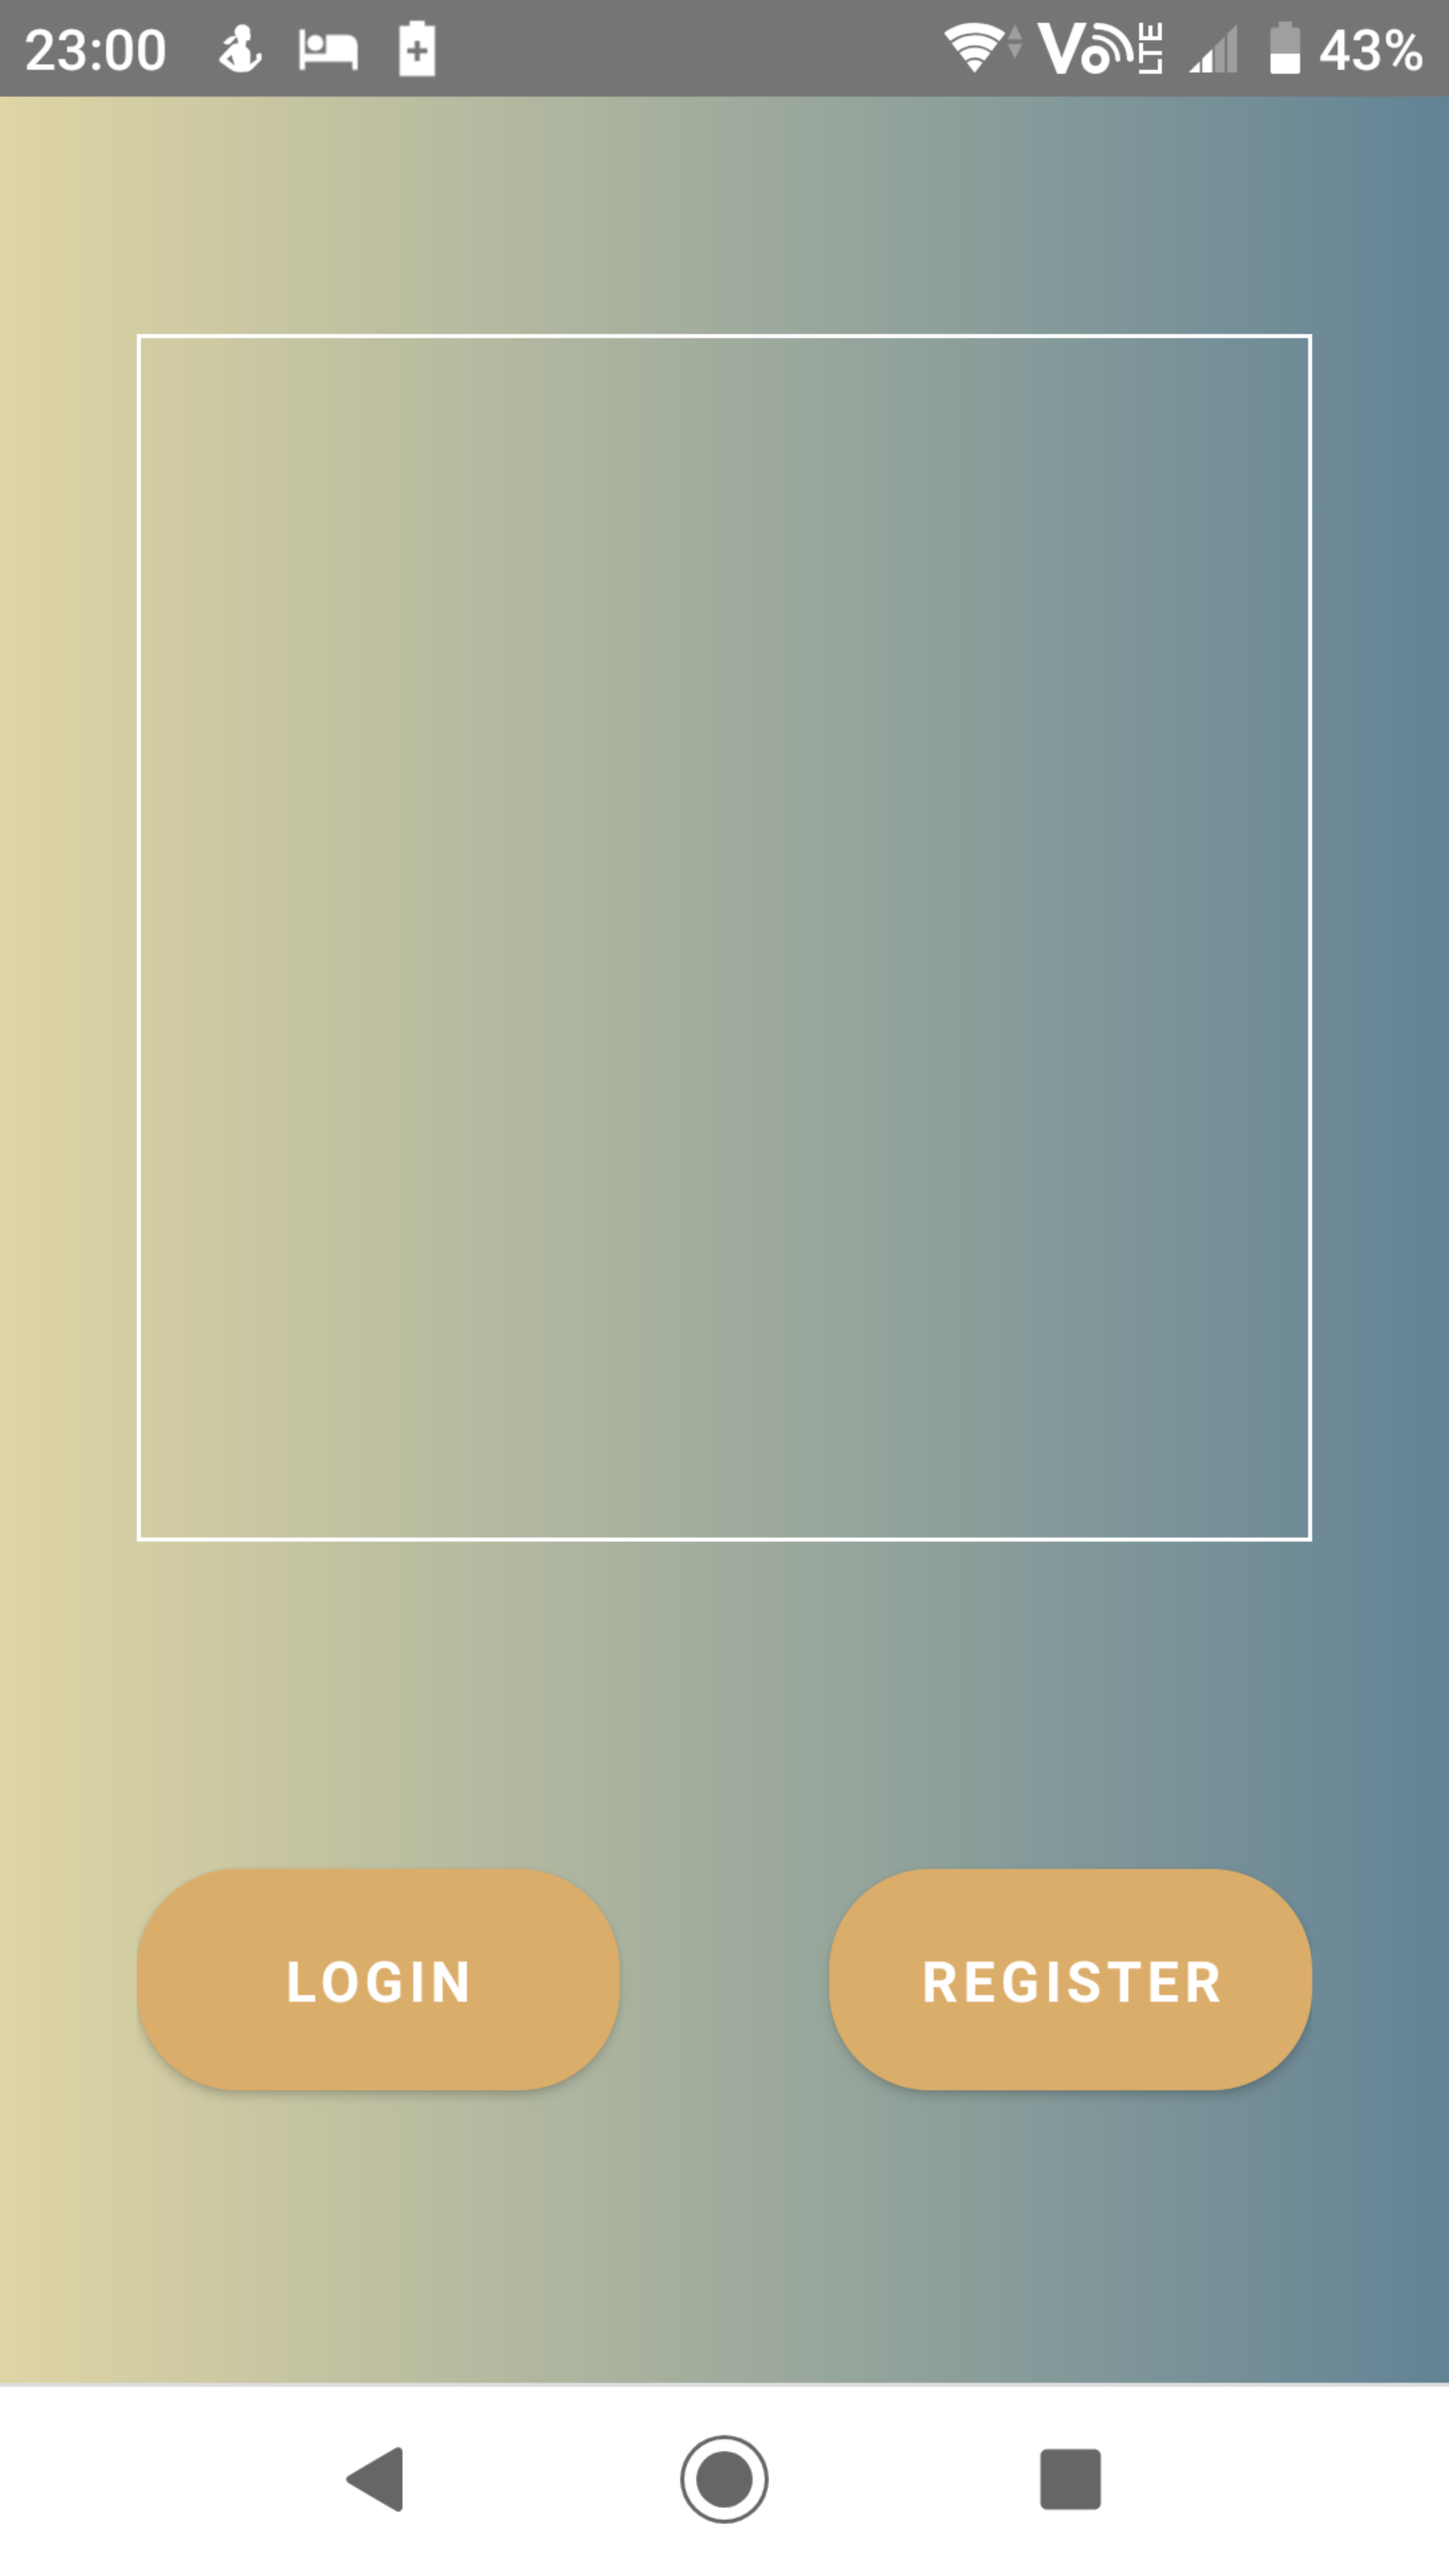
\includegraphics[width=0.5\linewidth]{images/mobile/first_view.png}
    \caption{Pierwszy widok po otworzeniu aplikacji mobilnej}
    \label{fig:test3_label}
\end{figure}

\section{Zarządzanie kontem}

\subsection{Rejestracja}
Aby móc korzystać z jakichkolwiek funkcjonalności serwisu, należy wpierw posiadać w nim swoje konto. \\

\textbf{Aplikacja webowa} \\
Znajdujemy w prawym górnym rogu przycisk \emph{Zarejestruj się} i go klikamy. Następnie uzupełniamy formularz z wymaganymi do utworzenia konta danymi.
Potem klikamy na przycisk \emph{Zarejestruj się}. Na adres mailowy podany w formularzu dostaniemy maila z linkiem potwierdzającym. Po kliknięciu na link, otrzymamy informację o specjalnie wygenerowanym dla nas loginie, za pomocą którego będziemy mogli się zalogować.

\begin{figure}[H]
    \centering
    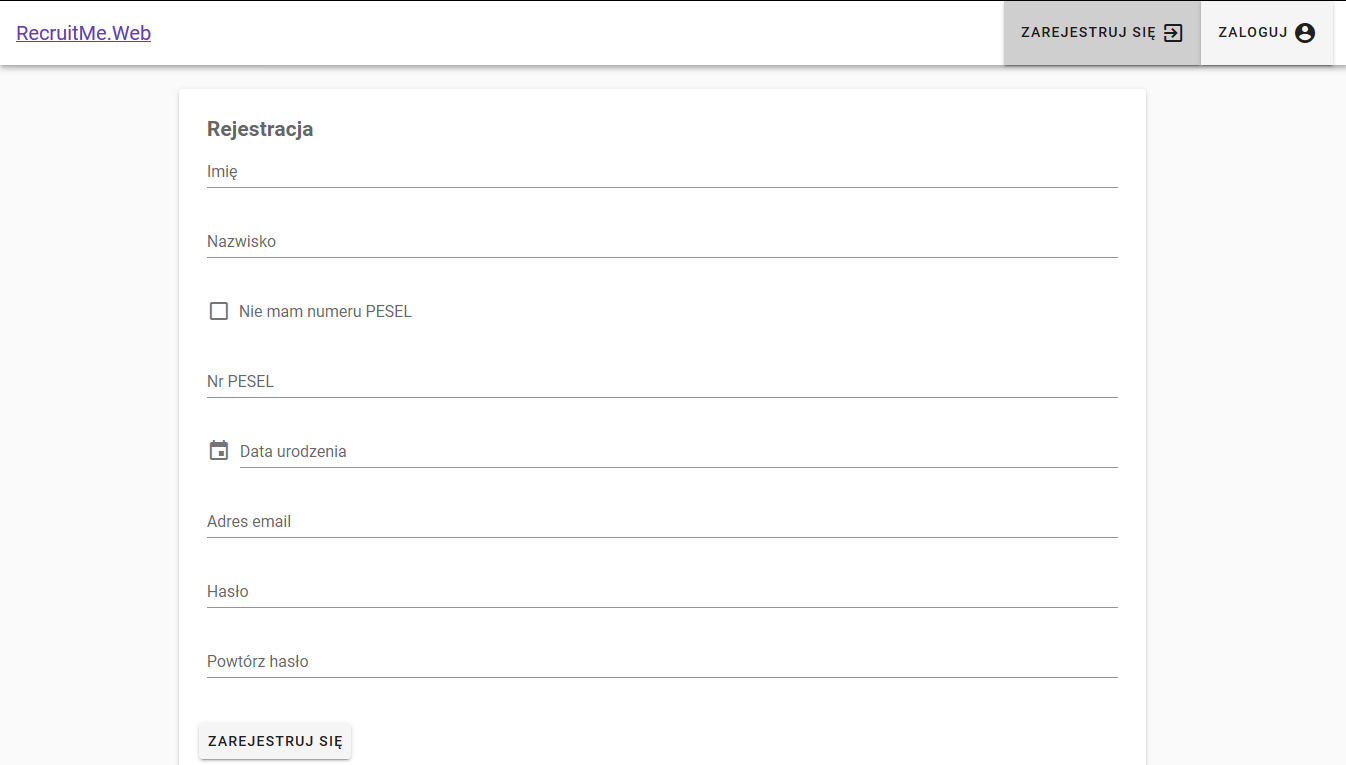
\includegraphics[width=1\linewidth]{images/web/register.png}
    \caption{Formularz rejestracji}
    \label{fig:test3_label}
\end{figure}

\textbf{Aplikacja mobilna} \\
Po uruchomieniu aplikacji, na głównym ekranie zobaczymy dwa przyciski - wybieramy ten z napisem \emph{Zarejestruj się}. Wypełniamy potrzebne dane do rejestracji. Po kliknięciu przycisku \emph{Zarejestruj}, dostaniemy potwierdzenie na górze ekranu o prośbie potwierdzenia maila.

\begin{figure}[H]
    \centering
    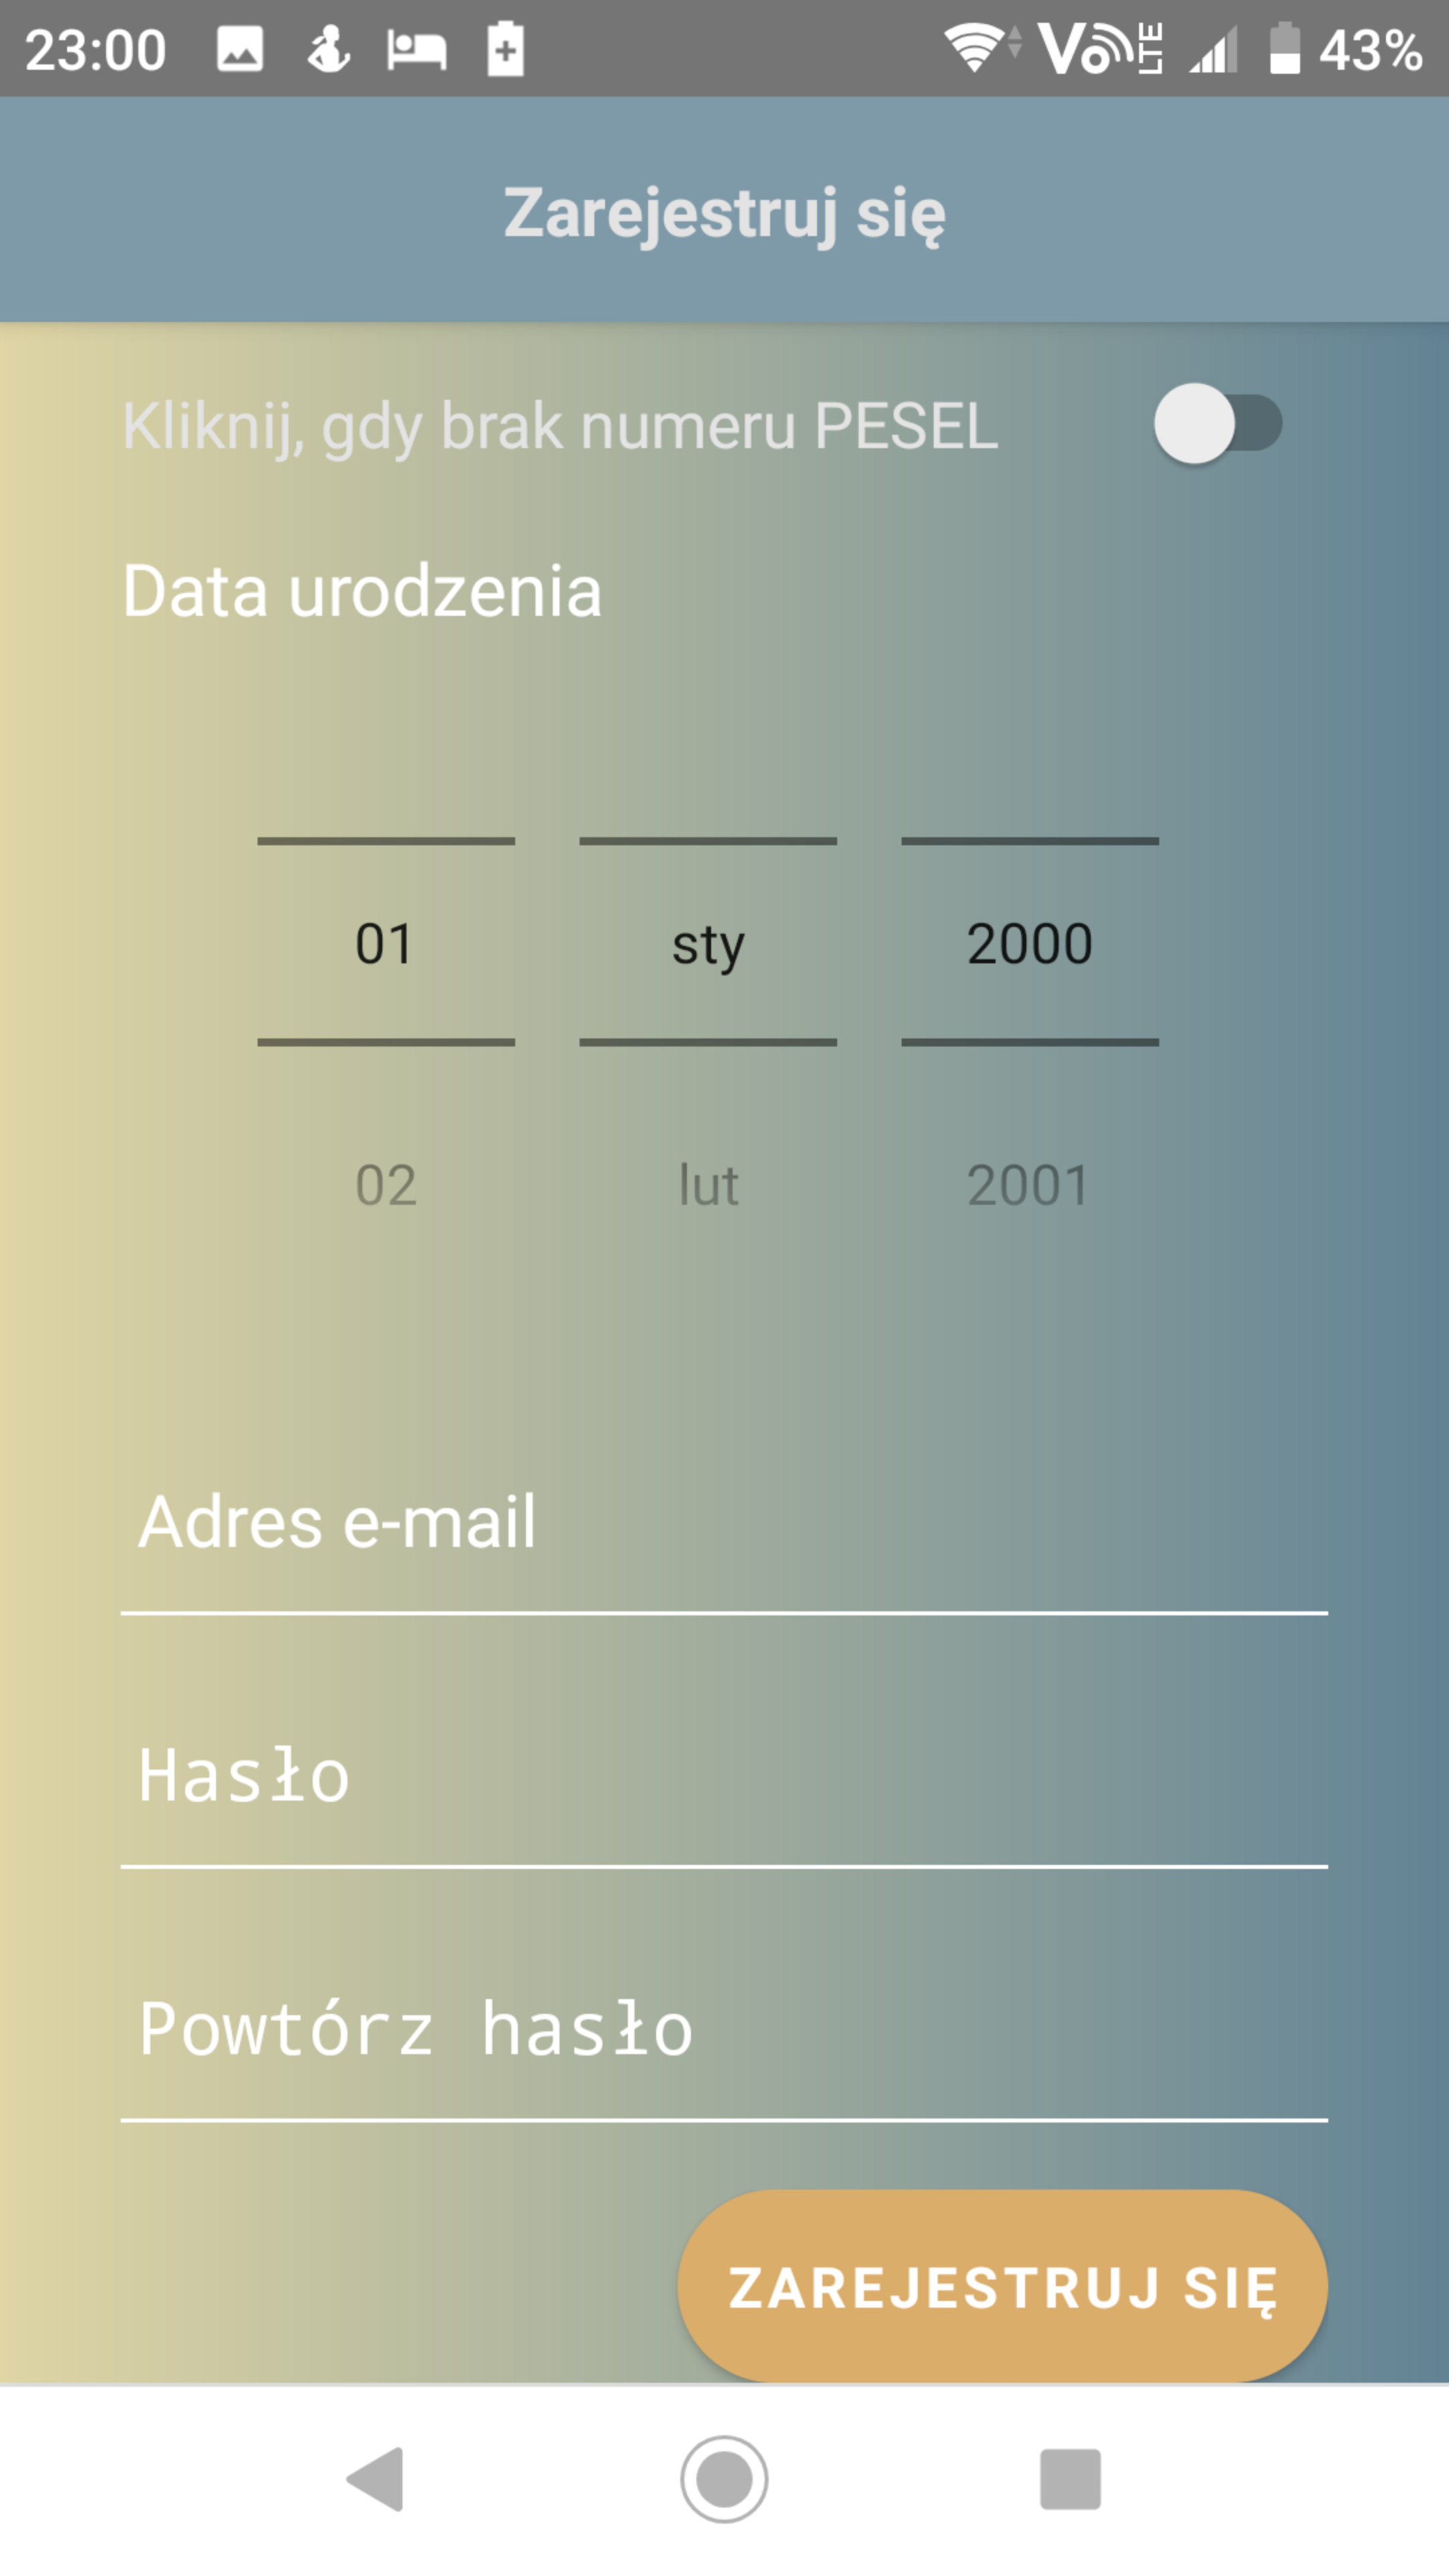
\includegraphics[width=0.45\linewidth]{images/mobile/register.png}
    \caption{Formularz rejestracji aplikacji mobilnej}
    \label{fig:test3_label}
\end{figure}

\subsection{Logowanie} 

\textbf{Aplikacja webowa} \\
Do ekranu logowania przechodzimy klikając w prawym górnym rogu na przycisk \emph{Zaloguj się}. Pojawi się nam formularz z polami login oraz hasło, które uzupełniamy danymi odpowiednio otrzymanymi i podanymi w procesie rejestracji.
Klikamy przycisk \emph{Zaloguj} i po chwili zostaniemy przeniesieni na stronę główną. W przypadku błędnych danych zostaniemy poinformowani odpowiednim komunikatem.
\begin{figure}[H]
    \centering
    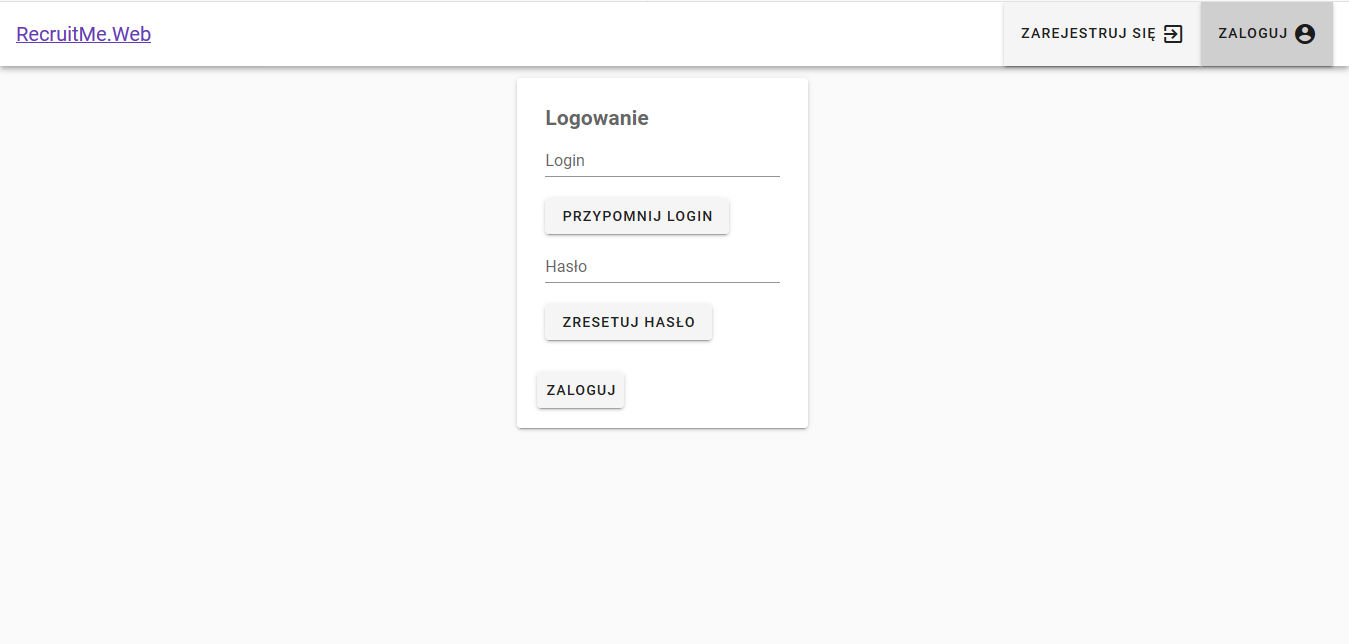
\includegraphics[width=1\linewidth]{images/web/login.png}
    \caption{Ekran logowania}
    \label{fig:test3_label}
\end{figure}

\textbf{Aplikacja mobilna} \\
Aby się zalogować, klikamy na głównym ekranie przycisk z napisem \emph{Logowanie}. W dostępne pola wpisujemy swój login, hasło i naciskamy \emph{Zaloguj się}. Jeżeli zostały wpisane poprawne dane, aplikacja przekieruje nas do widoku głównego.

\begin{figure}[H]
    \centering
    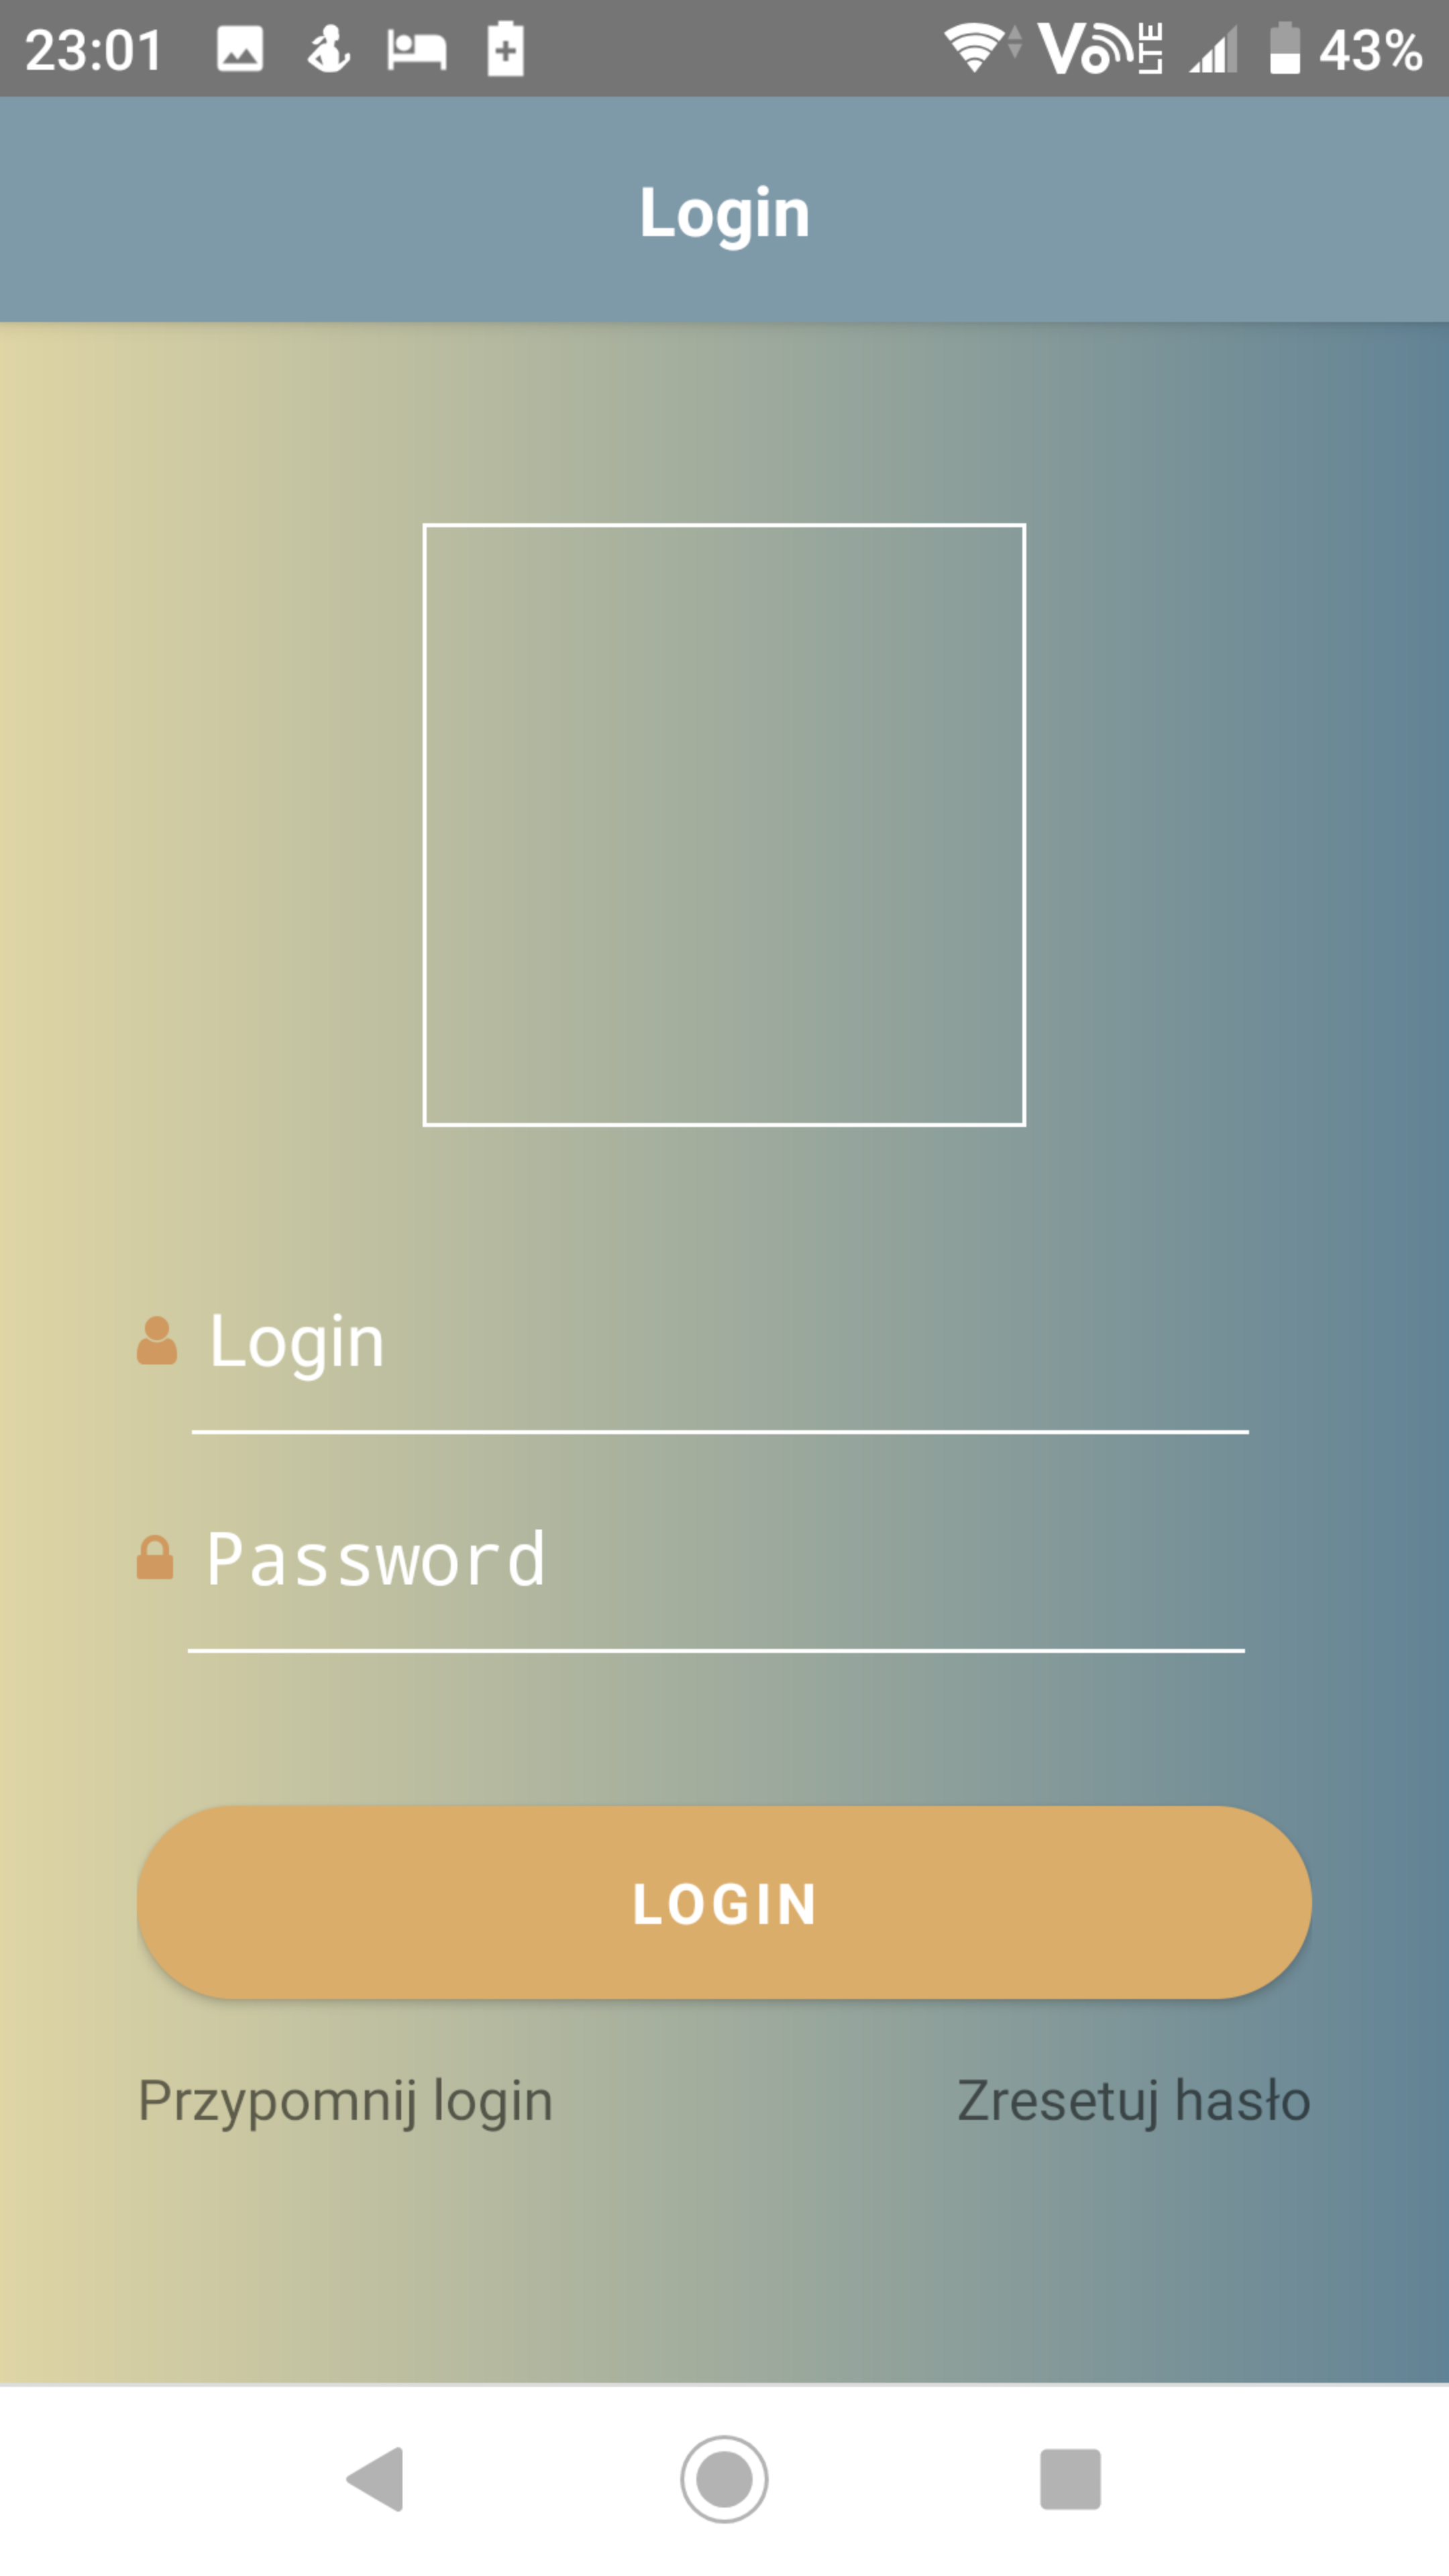
\includegraphics[width=0.45\linewidth]{images/mobile/login.png}
    \caption{Ekran logowania w aplikacji mobilnej}
    \label{fig:test3_label}
\end{figure}

\subsection{Przypomnienie loginu}
Przypomnienie loginu odbywa się w tym samym ekranie, co proces logowania się. \\

\textbf{Aplikacja webowa} \\
Należy kliknąć w prawym górnym rogu przeglądarki na przycisk \emph{Zaloguj się}, a następnie w przycisk \emph{Przypomnienie loginu}. Zostaniemy poproszeni o wpisanie swoich danych podanych w procesie rejestracji. Po kliknięciu w przycisk \emph{Sprawdź mój login}, na adres e-mail podany w rejestracji zostanie wysłany login.
\begin{figure}[H]
    \centering
    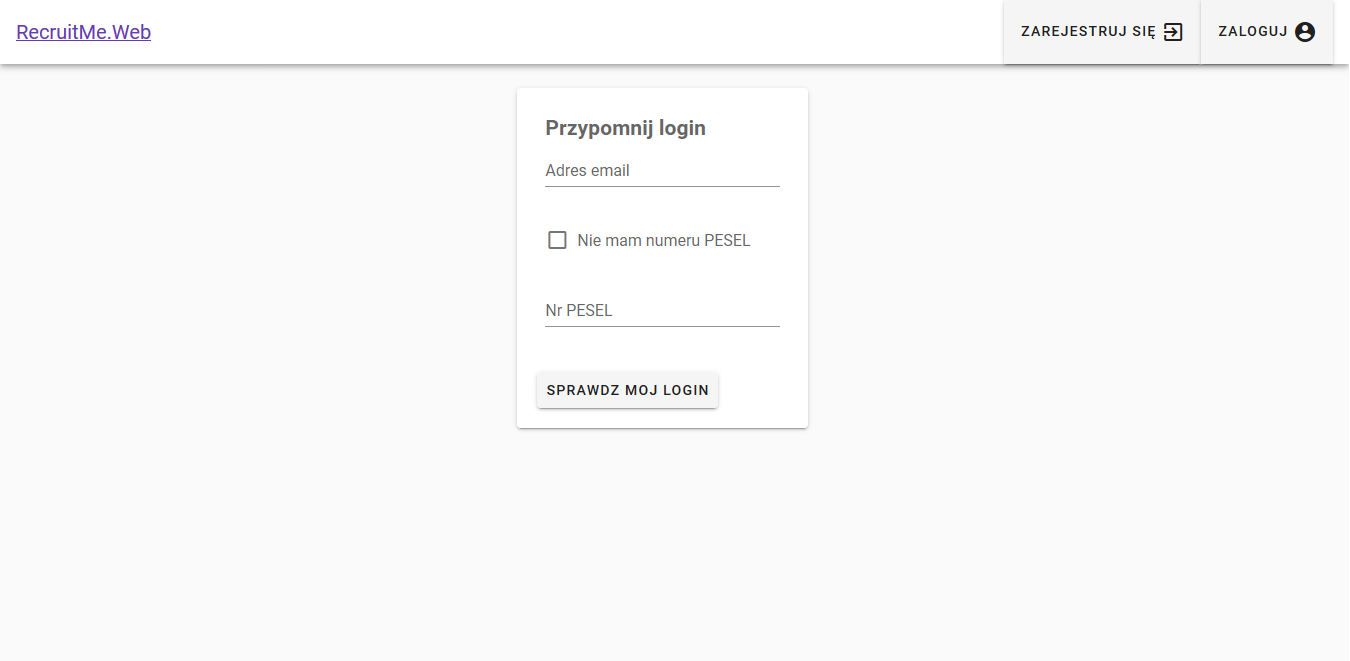
\includegraphics[width=1\linewidth]{images/web/remind_login.png}
    \caption{Formularz przypomnienia loginu}
    \label{fig:test3_label}
\end{figure}

\textbf{Aplikacja mobilna} \\
Przechodzimy do ekranu logowania, a następnie klikami napis \emph{Przypomnij login}. Następnie wypełniamy potrzebne dane. Po kliknięciu w przycisk \emph{Przypomnij login} na adres e-mail podany w rejestracji zostanie wysłany login.

\begin{figure}[H]
    \centering
    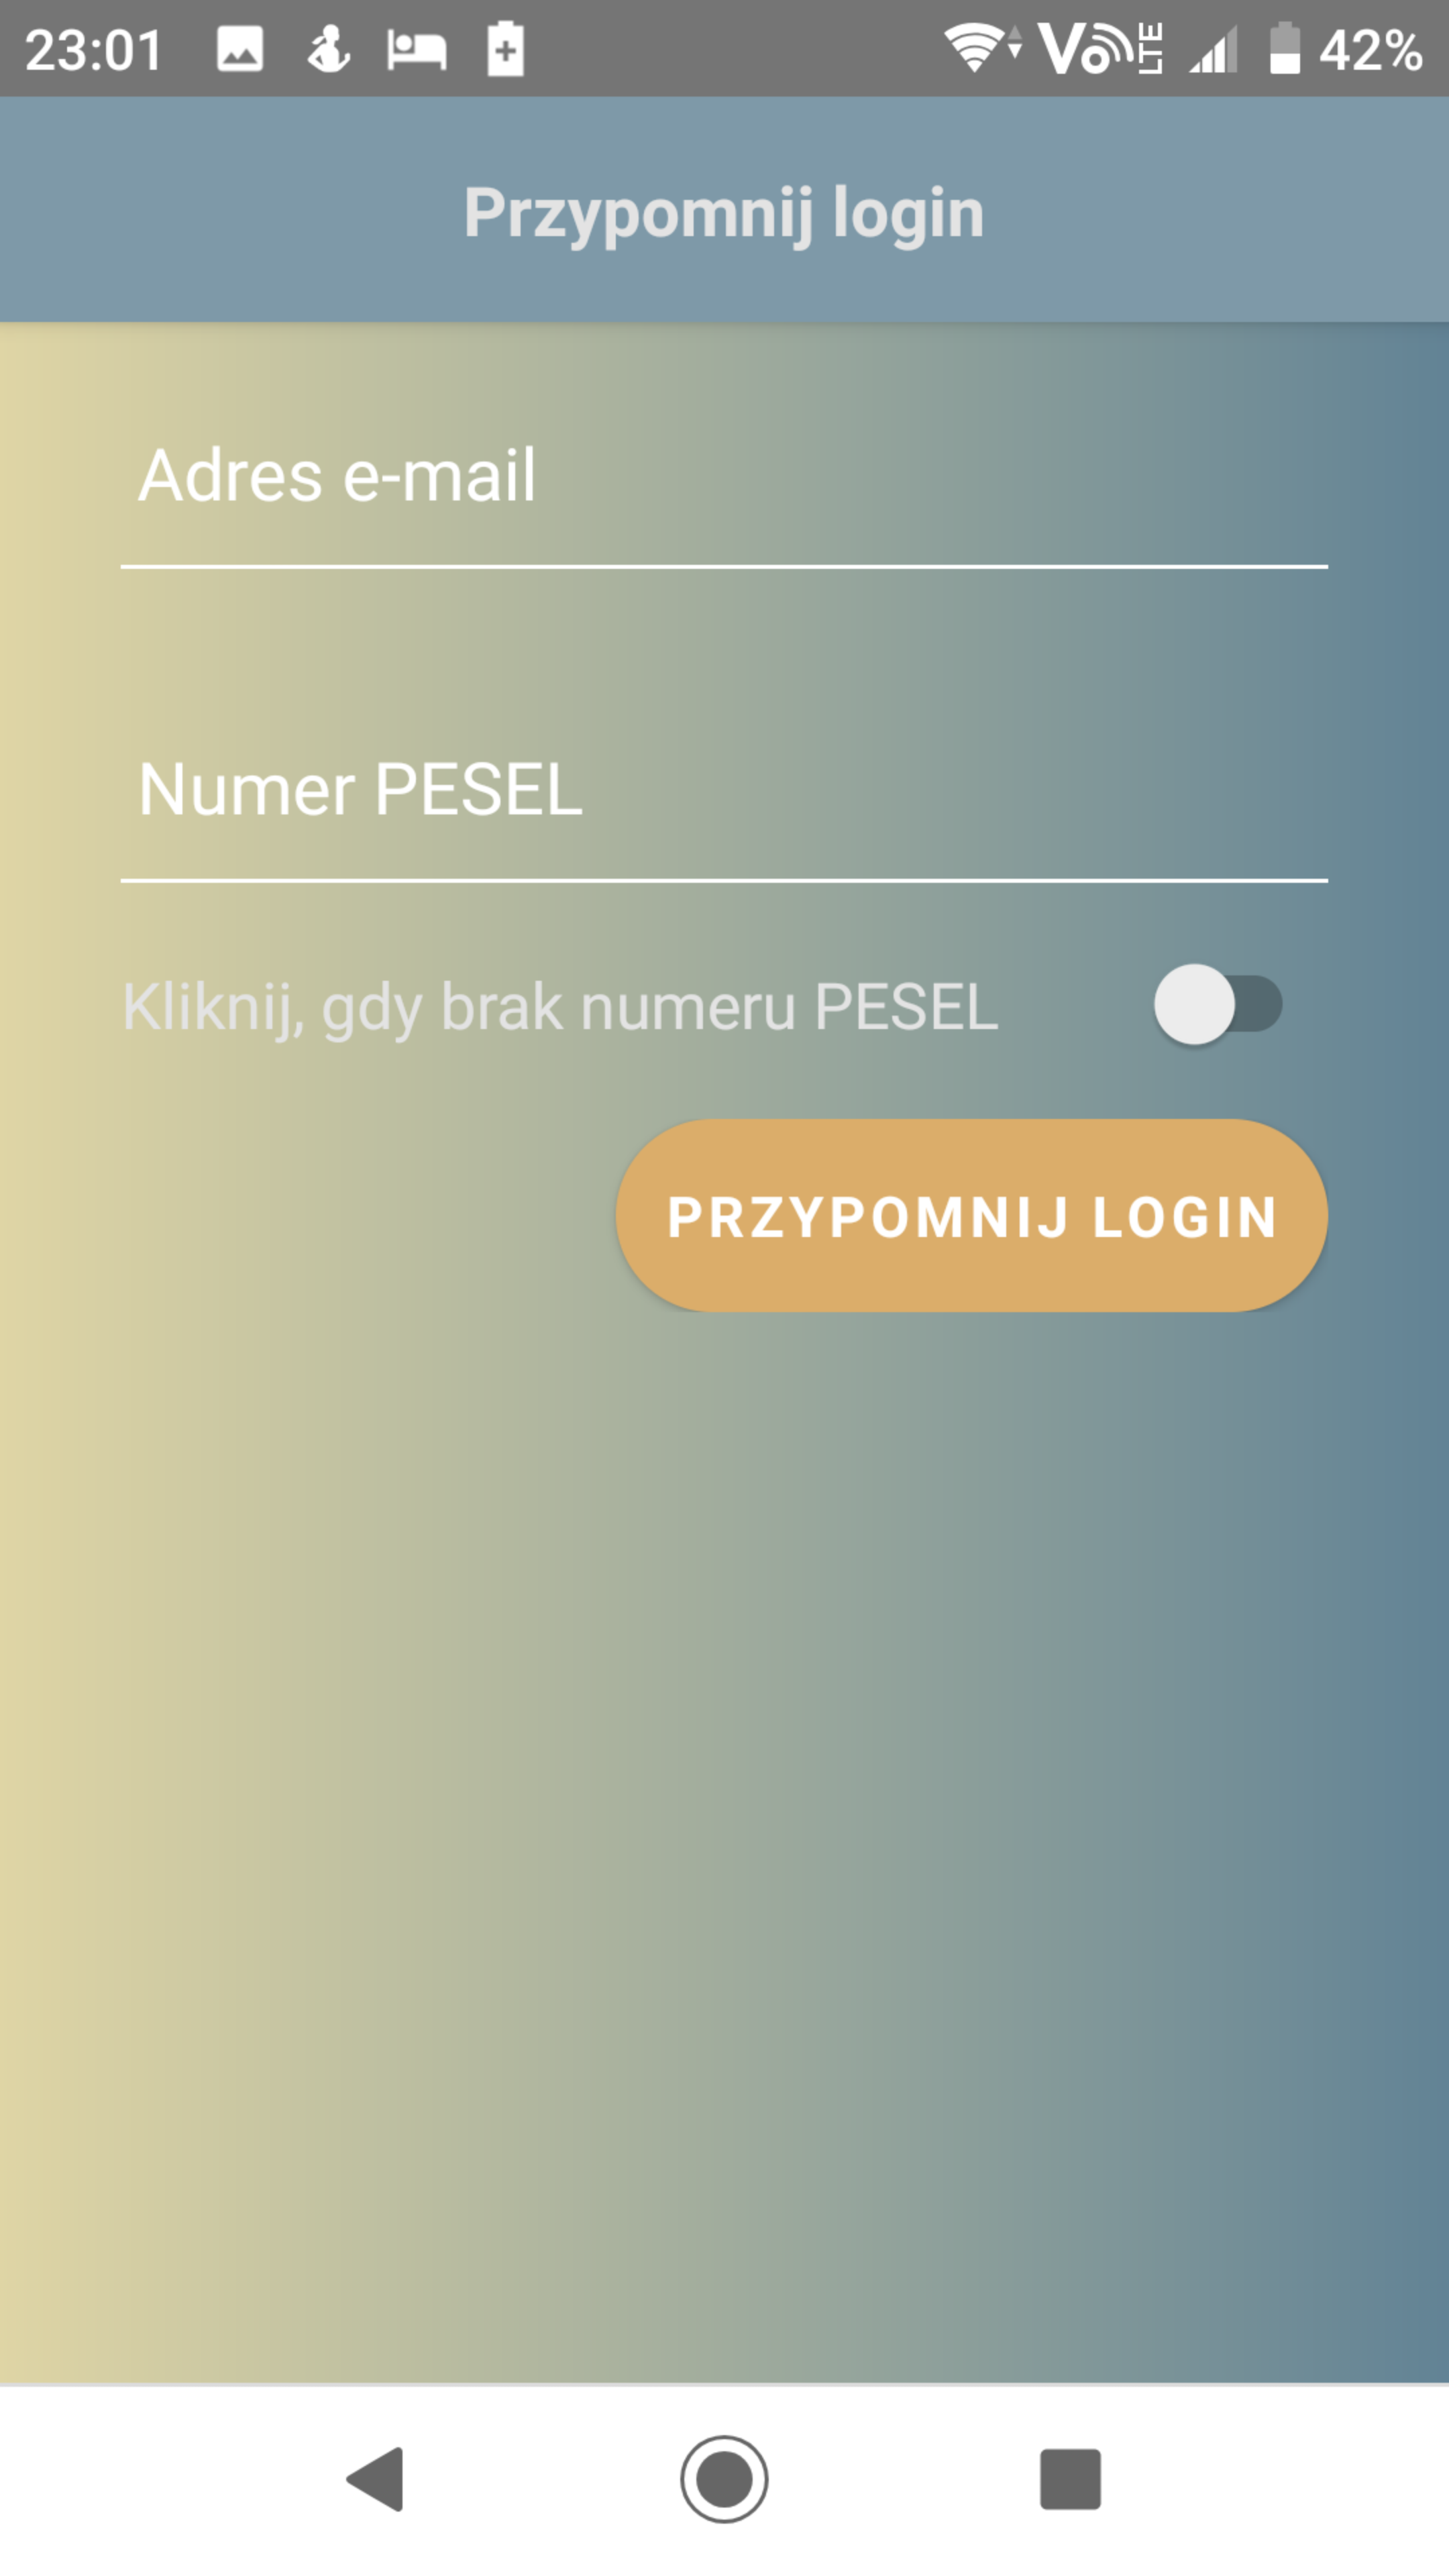
\includegraphics[width=0.45\linewidth]{images/mobile/remind_login.png}
    \caption{Formularz przypomnienia loginu w aplikacji mobilnej}
    \label{fig:test3_label}
\end{figure}

\subsection{Przypomnienie hasła}
Przypomnienie hasła odbywa się w tym samym ekranie, co proces logowania się.
\\

\textbf{Aplikacja webowa} \\
Należy kliknąć w prawym górnym rogu przeglądarki na przycisk \emph{Zaloguj się}, a następnie w przycisk \emph{Przypomnienie hasła}. Zostaniemy poproszeni o wpisanie swoich danych podanych w procesie rejestracji. Po kliknięciu w przycisk \emph{Resetuj hasło}, na adres e-mail podany w rejestracji zostanie wysłany link umożliwiający zmianę hasła. Link umożliwia przeniesienie do formularza zmiany hasła, gdzie zostaniemy poproszeni o wpisanie dwa razy tego samego hasła. Po kliknięciu w przycisk \emph{Resetuj hasło}, dostaniemy ekran potwierdzający i od tej pory możemy się logować nowym hasłem.
\begin{figure}[H]
    \centering
    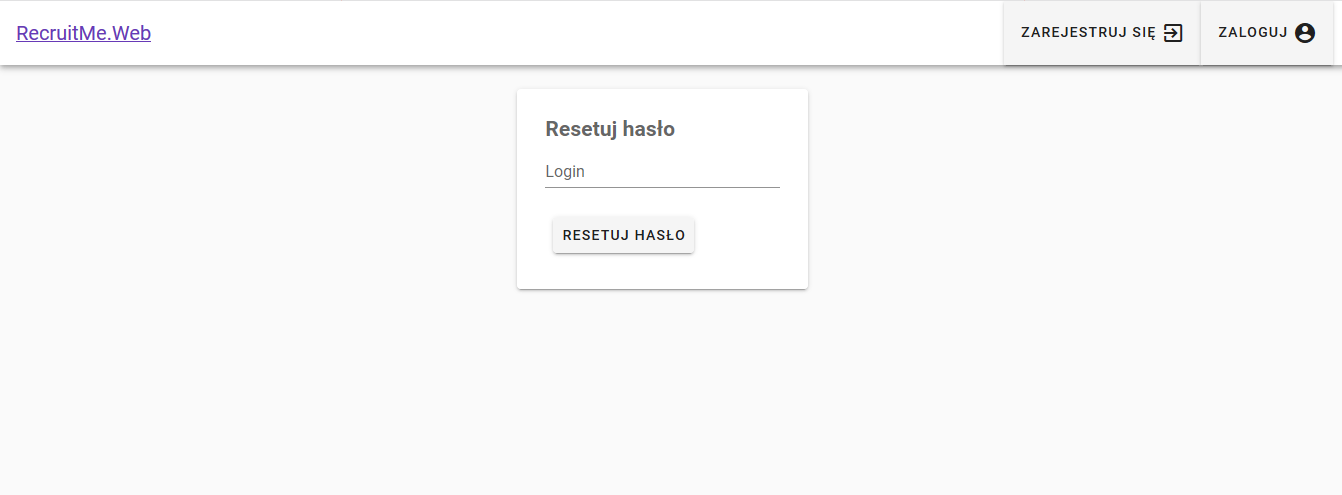
\includegraphics[width=1\linewidth]{images/web/reset_password.png}
    \caption{Formularz przypomnienia hasła}
    \label{fig:test3_label}
\end{figure}

\textbf{Aplikacja mobilna} \\
Przechodzimy do ekranu logowania i klikamy w tekst \emph{Przypomnij hasło}.
Wpisujemy potrzebne dane, a następnie klikamy w przycisk \emph{Zresetuj hasło}. Na adres e-mail podany w rejestracji zostanie wysłany link umożliwiający zmianę hasła.
Dalej odnawiamy hasło przez aplikację webową.

\begin{figure}[H]
    \centering
    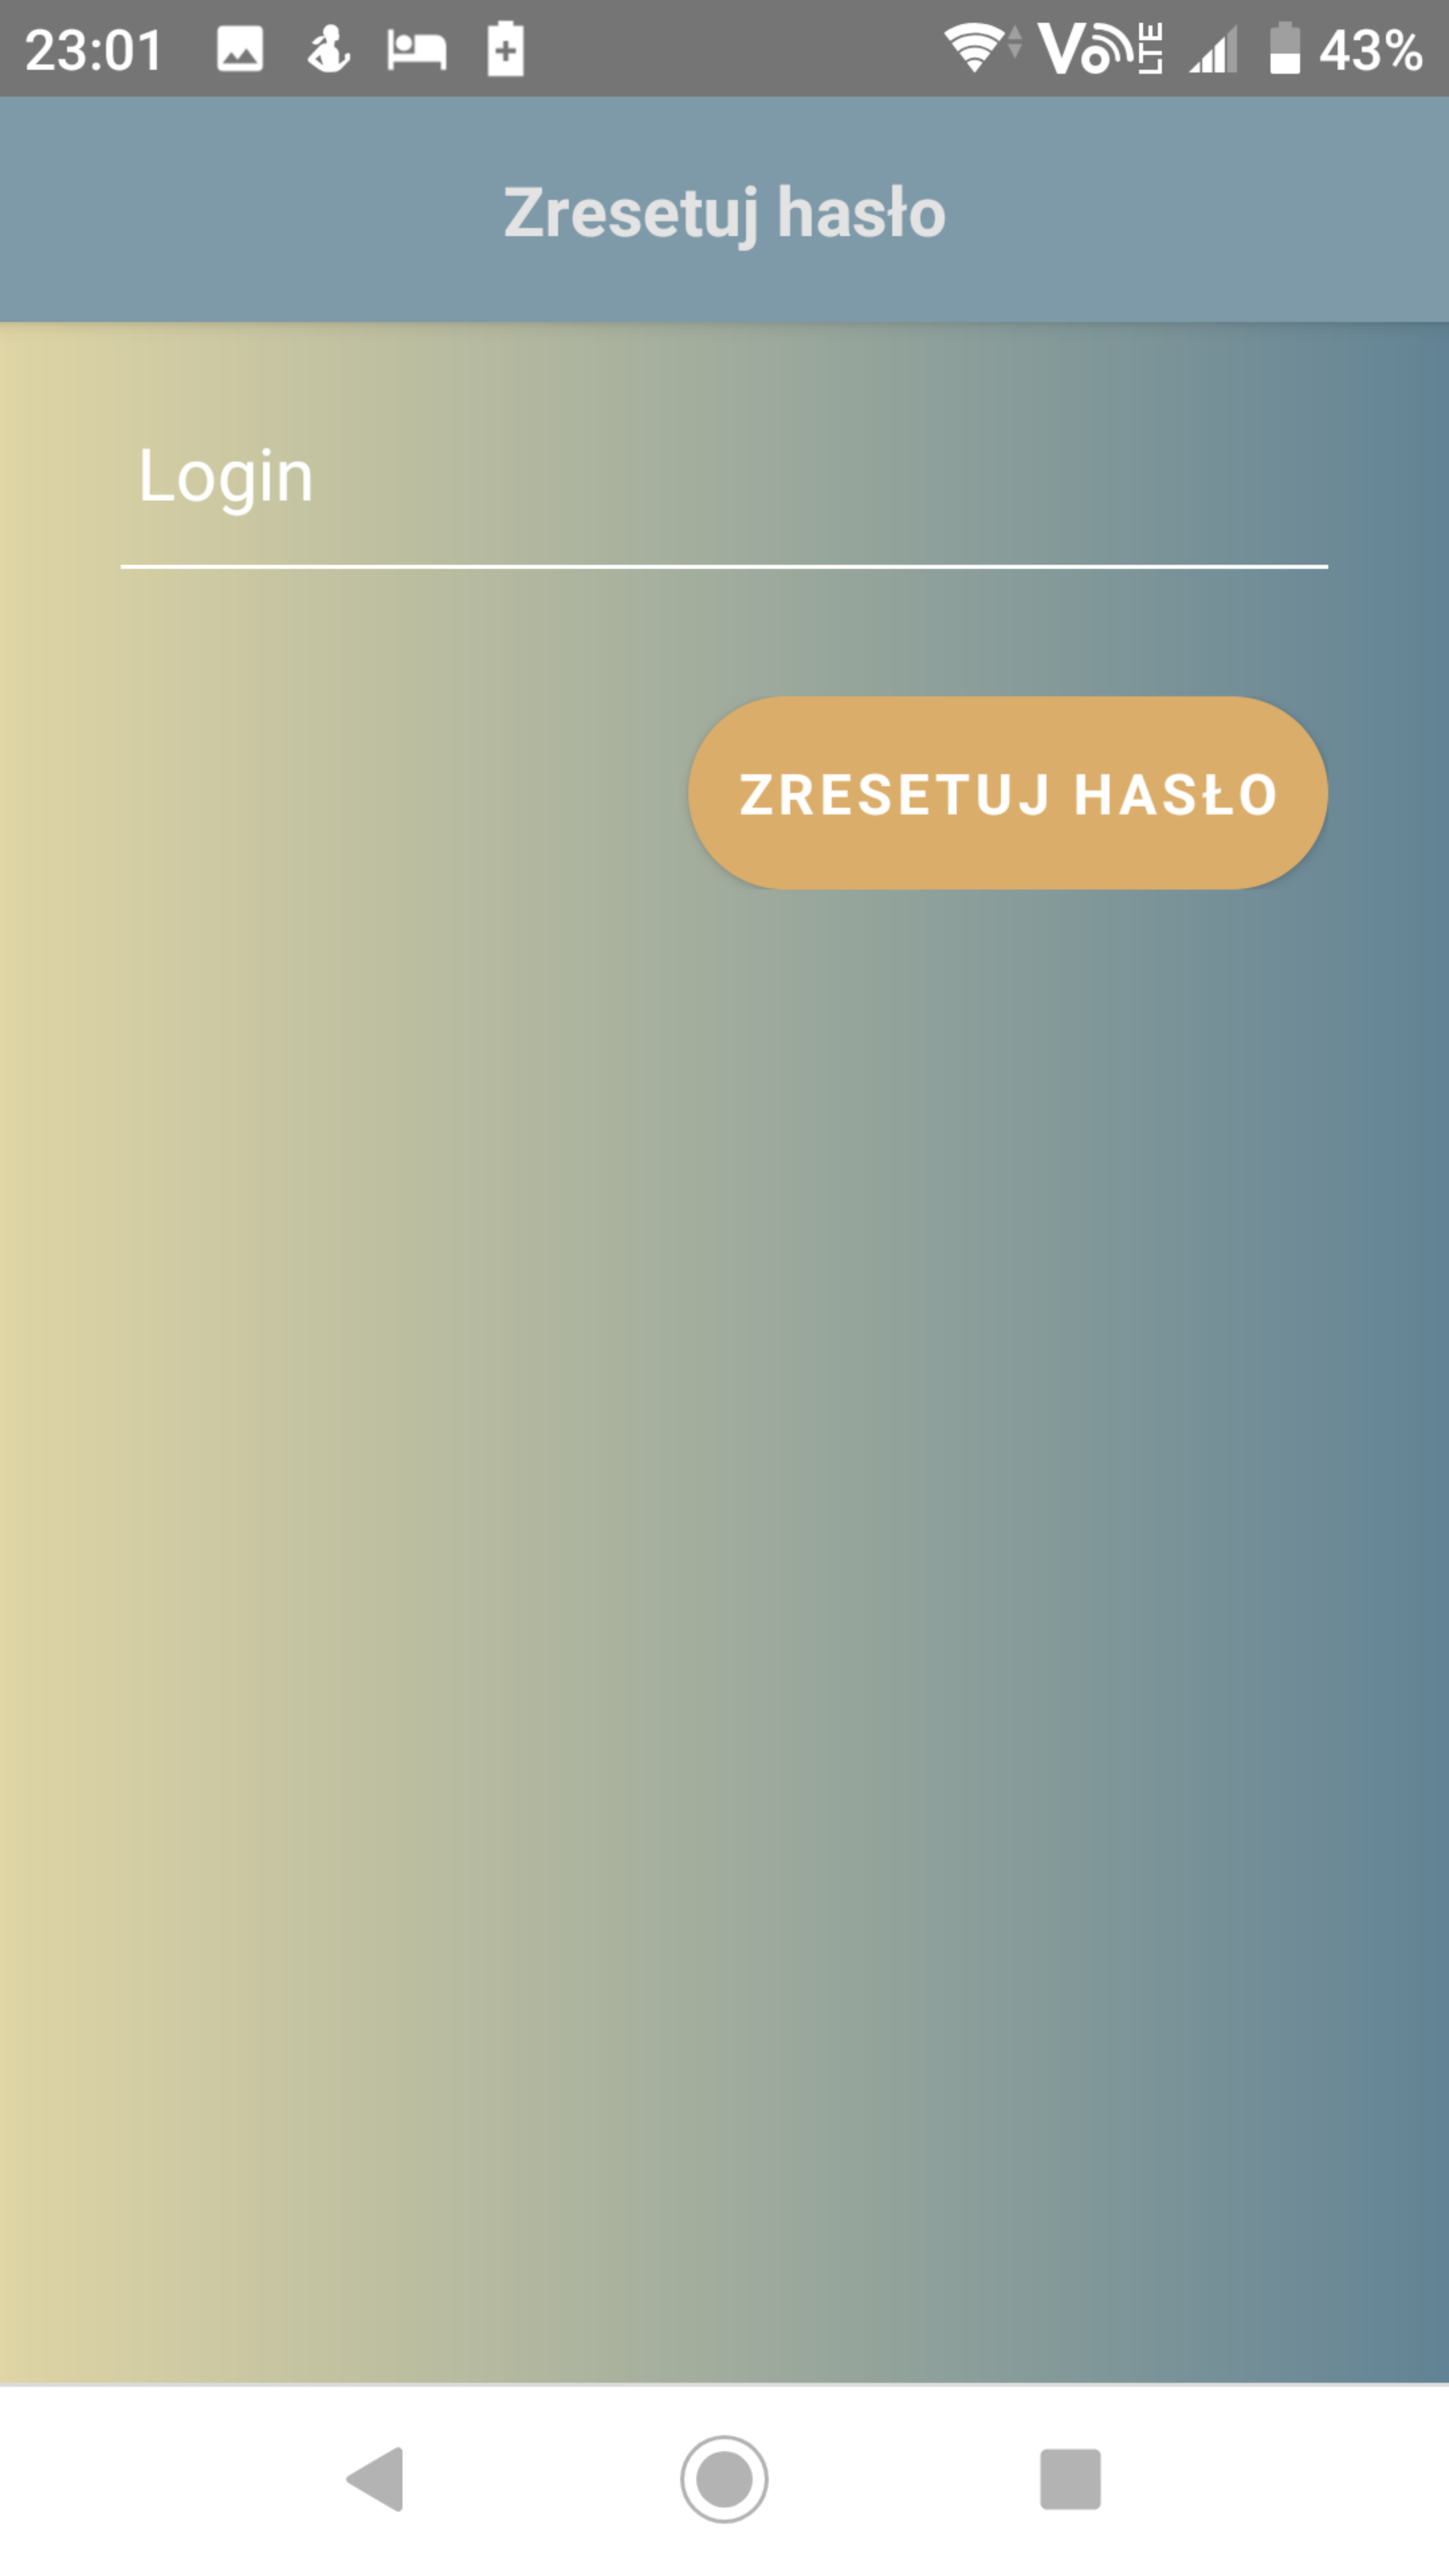
\includegraphics[width=0.45\linewidth]{images/mobile/reset_password.png}
    \caption{Formularz przypomnienia hasła w aplikacji mobilnej}
    \label{fig:test3_label}
\end{figure}

\section{Profil kandydata}

\subsection{Ustawianie zdjęcia profilowego}
Kandydat, by ułatwić weryfikację przez nauczycieli na egzaminie, może wysłać do systemu swoje zdjęcie. \\

\textbf{Aplikacja webowa} \\
Po zalogowaniu, klikamy na przycisk \emph{Profil} w prawym górnym rogu. Po prawej stronie będziemy widzieli kwadrat z domyślnym zdjęciem kandydata oraz dwoma przyciskami pod nim. Możemy wybrać zdjęcie z naszego komputera i wgrać do systemu, klikając na domyślne zdjęcie. Ewentualnie możemy kliknąć przycisk \emph{Zrób zdjęcie teraz}, aby skorzystać z kamerki internetowej, aby zrobić sobie zdjęcie. W dowolnym przypadku należy potwierdzić swoją decyzję klikając przycisk \emph{Zapisz zdjęcie}.
\begin{figure}[H]
    \centering
    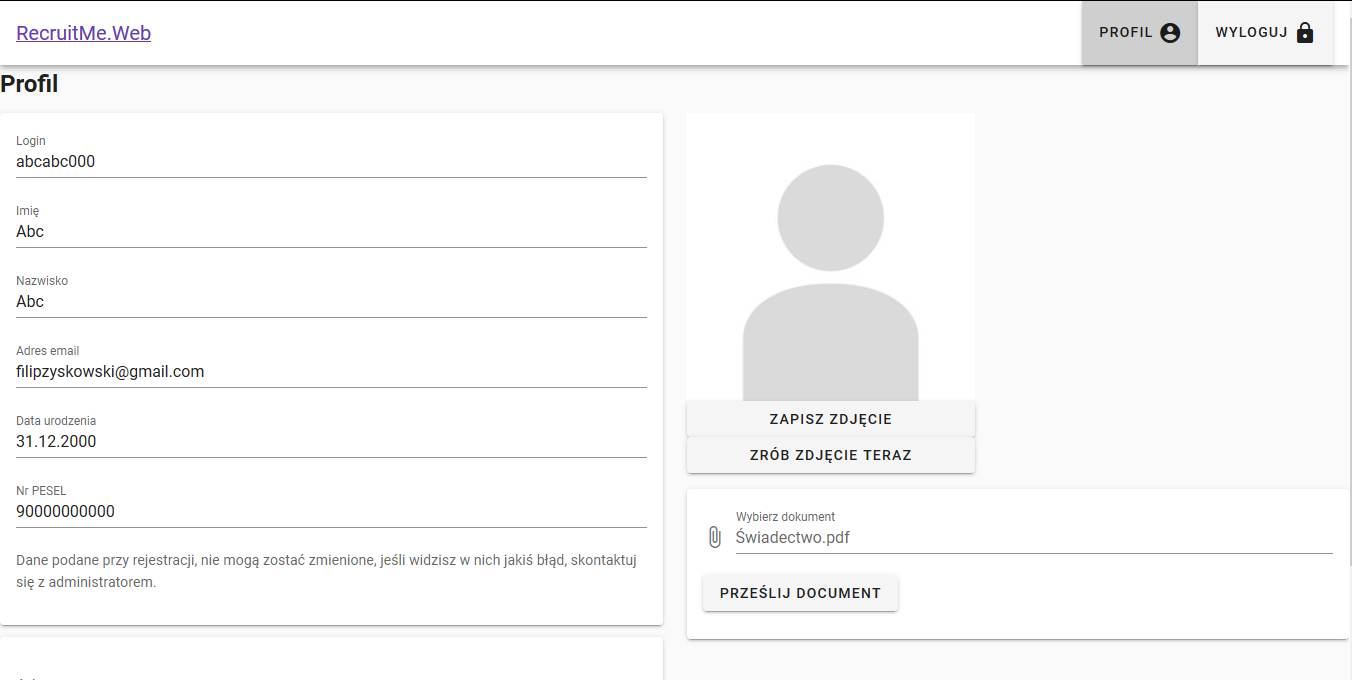
\includegraphics[width=1\linewidth]{images/web/profil.png}
    \caption{Ekran profilu kandydata}
    \label{fig:test3_label}
\end{figure}

\textbf{Aplikacja mobilna} \\
Po zalogowaniu klikamy na ikonę trzech białych pasków w lewym górnym rogu aplikacji lub przeciągamy palec z lewej do prawej ekranu telefonu, aby wyciągnąć menu aplikacji. Tam należy kliknąć \emph{Ustawienia}. Następnie należy kliknąć jedno z dwóch przycisków: \emph{Zrób zdjęcie} lub \emph{Wybierz z galerii}. Naciśnięcie pierwszego przycisku po raz pierwszy sprawi, że zostanie wyświetlona prośba o zgodę na użycie aparatu komórki oraz zgodę na użycie multimediów. Nieudzielenie zgody uniemożliwi wysłanie zdjęcia na serwer aplikacji. Aplikacja po zrobieniu zdjęcia przez użytkownika automatycznie wysyła je na serwer. Podobnie się staje po kliknięciu drugiego przycisku - wyświetla się prośba o udzielenie zgody na dostęp do plików, kandydat wybiera zdjęcie i zdjęcie zostaje zapisane.
\begin{figure}[H]
    \centering
    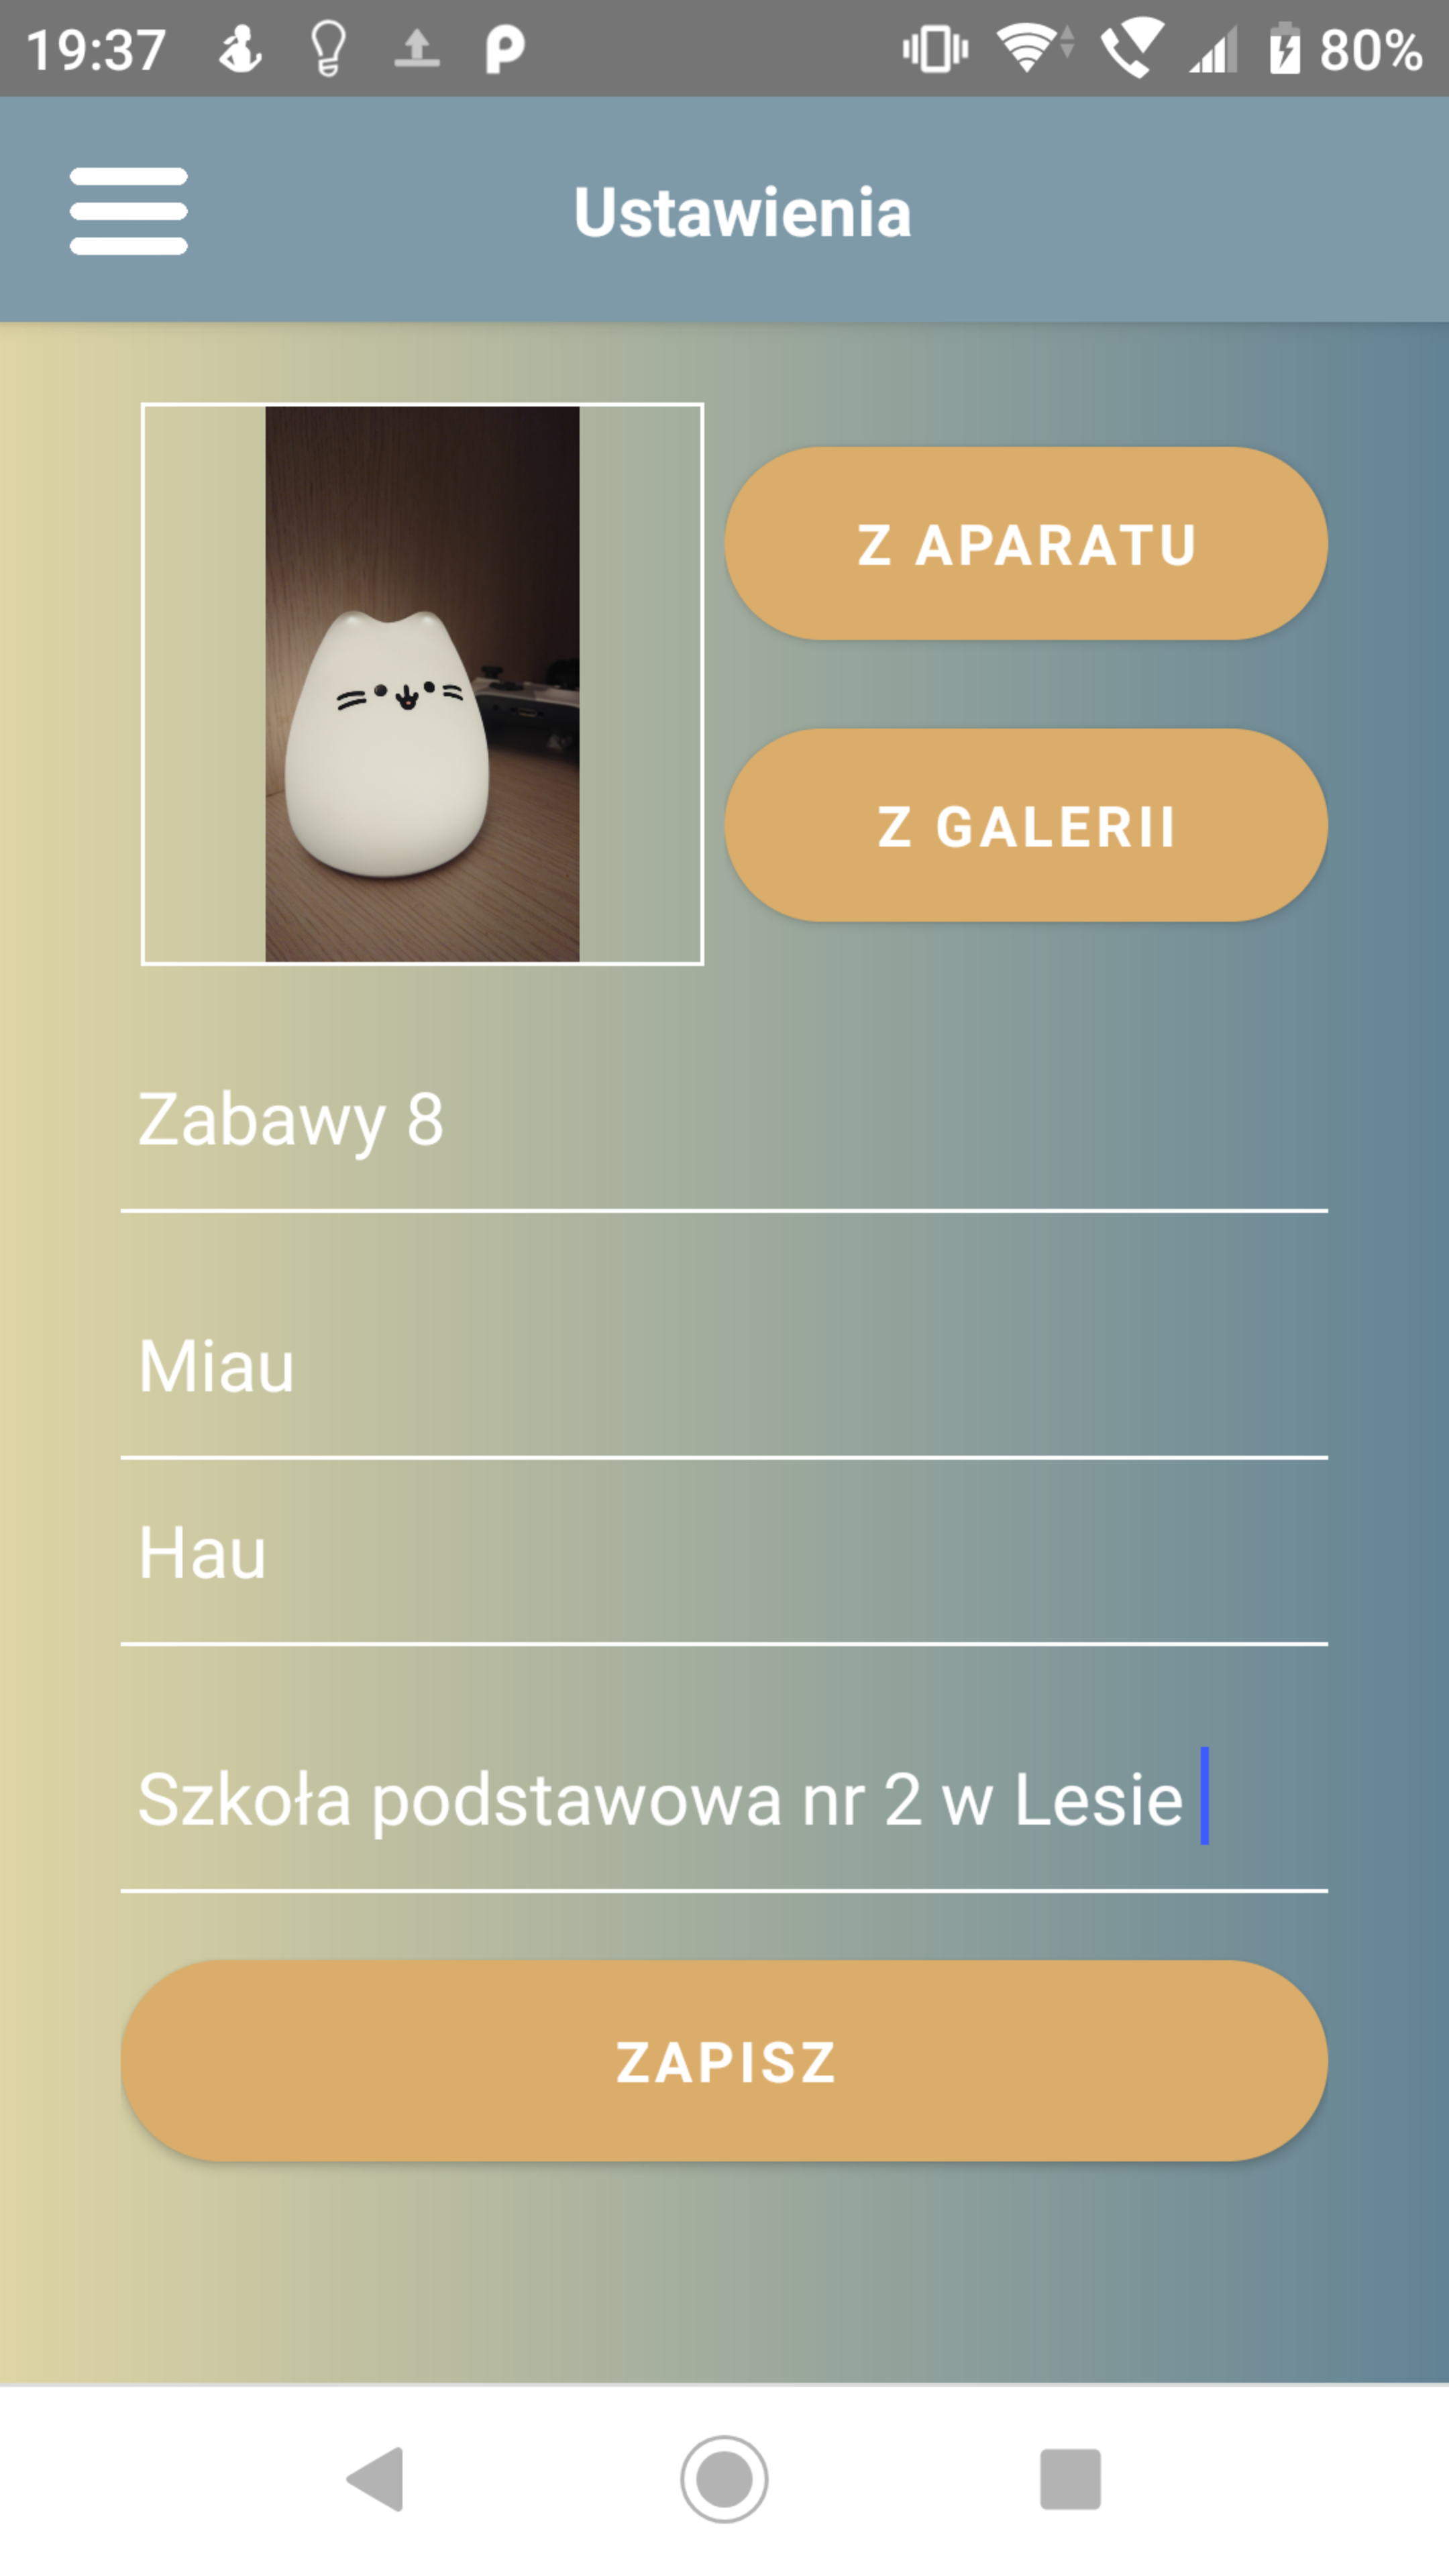
\includegraphics[width=0.45\linewidth]{images/mobile/candidate_settings.png}
    \caption{Ekran profilu kandydata w aplikacji mobilnej}
    \label{fig:test3_label}
\end{figure}

\subsection{Dodawanie dodatkowych danych}
Kandydat zostanie poproszony o wypełnienie dodatkowych danych takich jak imiona rodziców przed zapisaniem na egzaminy. Zarówno w aplikacji webowej jak i mobilnej, wpisywanie dodatkowych danych jest umieszczone w tym samym ekranie co ustawianie zdjęcia profilowego. \\

\textbf{Aplikacja webowa} \\
Poniżej danych podstawowych użytkownika w profilu kandydata znajduje się formularz danych dodatkowych. Użytkownik po wypełnieniu danych powinien kliknąc przycisk \emph{Zapisz dane}, by dane prawidłowo zapisały się w serwisie.
\begin{figure}[H]
    \centering
    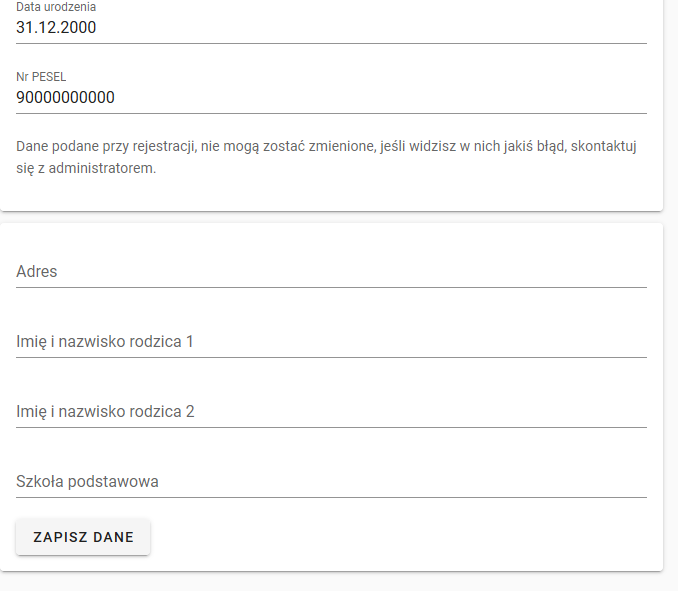
\includegraphics[width=1\linewidth]{images/web/additional_data.png}
    \caption{Uzupełnianie dodatkowych danych}
    \label{fig:test3_label}
\end{figure}

\textbf{Aplikacja mobilna} \\
Poniżej zdjęcia profilowego użytkownika w profilu kandydata znajduje się formularz danych dodatkowych. Użytkownik po wypełnieniu danych powinien kliknąc przycisk \emph{Zapisz}, by dane prawidłowo zapisały się w serwisie. O sukcesie bądź niepowodzeniu kandydat zostanie poinformowany odpowiednim komunikatem, który się pojawi u góry ekranu.

\section{Płatności}
Przed zapisaniem się na egzaminy wymagane jest uiszczenie opłaty rekrutacyjnej. By to ułatwić, aplikacja wystawia dogodny interfejs użytkownika umożliwiający łatwy transfer środków. Po realizacji płatności przez bramkę płatniczą, system automatycznie rejestruje kandydata na wszystkie dostępne w rejestracji egzaminy.

\subsection{Dokonanie płatności}
Dokonanie płatności przebiega w specjalnym ekranie statusu płatności \\

\textbf{Aplikacja webowa} \\
Aby dokonać płatności, należy przejść do ekranu statusu płatności, znajdującego się w prawym górnym rogu ekranu w zakładce \emph{Płatności}.
Jeżeli nie opłaciliśmy kwoty rekrutacyjnej, zobaczymy informację o braku zaksięgowanej płatności i przycisk w prawym dolnym rogu z możliwością dokonania płatności.
\begin{figure}[H]
    \centering
    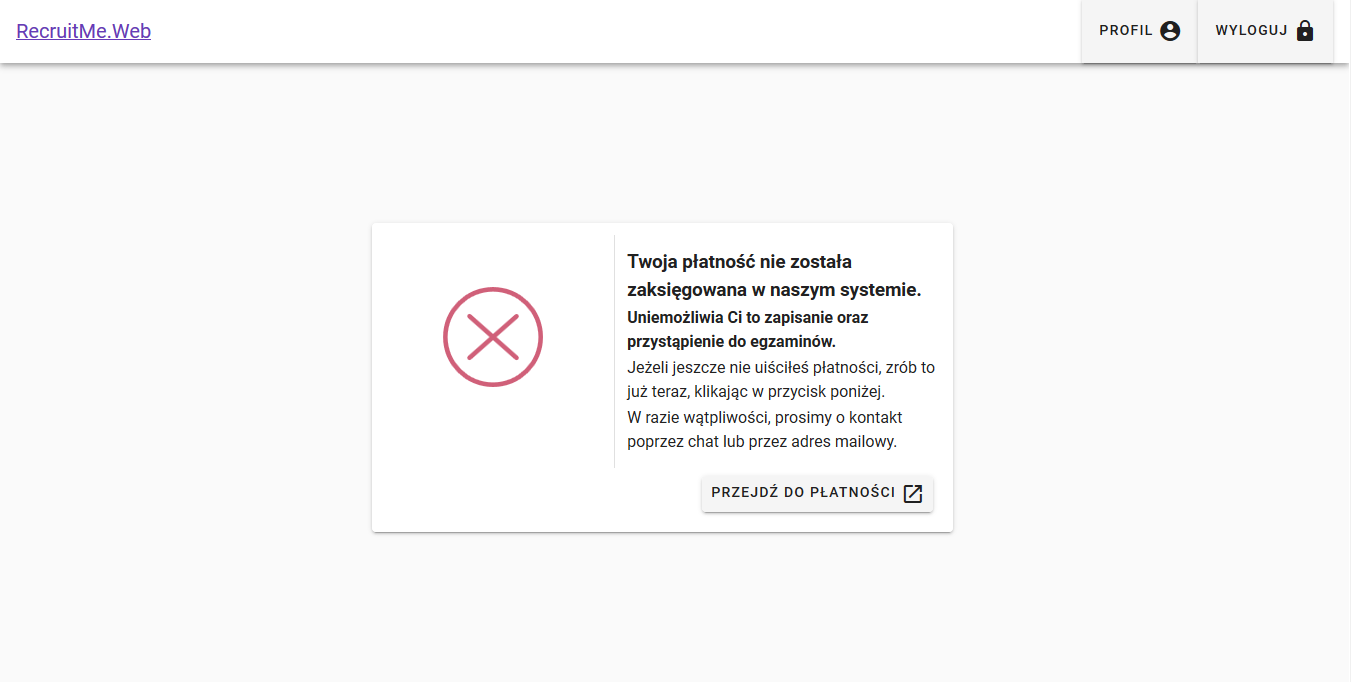
\includegraphics[width=1\linewidth]{images/web/payments.png}
    \caption{Ekran statusu płatności}
    \label{fig:test3_label}
\end{figure}
Po kliknięciu zostaniemy przekierowani na stronę bramki płatniczej Dotpay. Wybieramy interesującą nas metodę płatności i podajemy swoje dane. Klikamy przycisk \emph{Zapłać}, by zatwierdzić płatność. W zależności od wybranej metody płatności, możemy być również przeniesieni na stronę naszego banku, by uzupełnić dodatkowe dane potrzebne do procesu. Następnie, gdy nie będzie żadnych błędów, dostaniemy informację od bramki płatniczej o udanej transakcji. Dostaniemy także przycisk umożliwiający powrót do naszego systemu.
W zależności od wybranej metody płatności, proces weryfikacji może potrwać nawet do kilku dni roboczych. \\

\textbf{Aplikacja mobilna} \\
Klikamy trzy białe paski w lewym górnym robu albo wyciągamy z lewej strony ekran menu i wybieramy \emph{Płatności}. Jeżeli nie opłaciliśmy kwoty rekrutacyjnej, zobaczymy informację o braku zaksięgowanej płatności i przycisk w prawym dolnym rogu z możliwością dokonania płatności.
Potem analogicznie do aplikacji webowej przechodzimy przez proces bramki płatniczej. Przy powrocie do naszego serwisu zostaniemy skierowani z powrotem do aplikacji mobilnej.
W zależności od wybranej metody płatności, proces weryfikacji może potrwać nawet do kilku dni roboczych.

\begin{figure}[H]
    \centering
    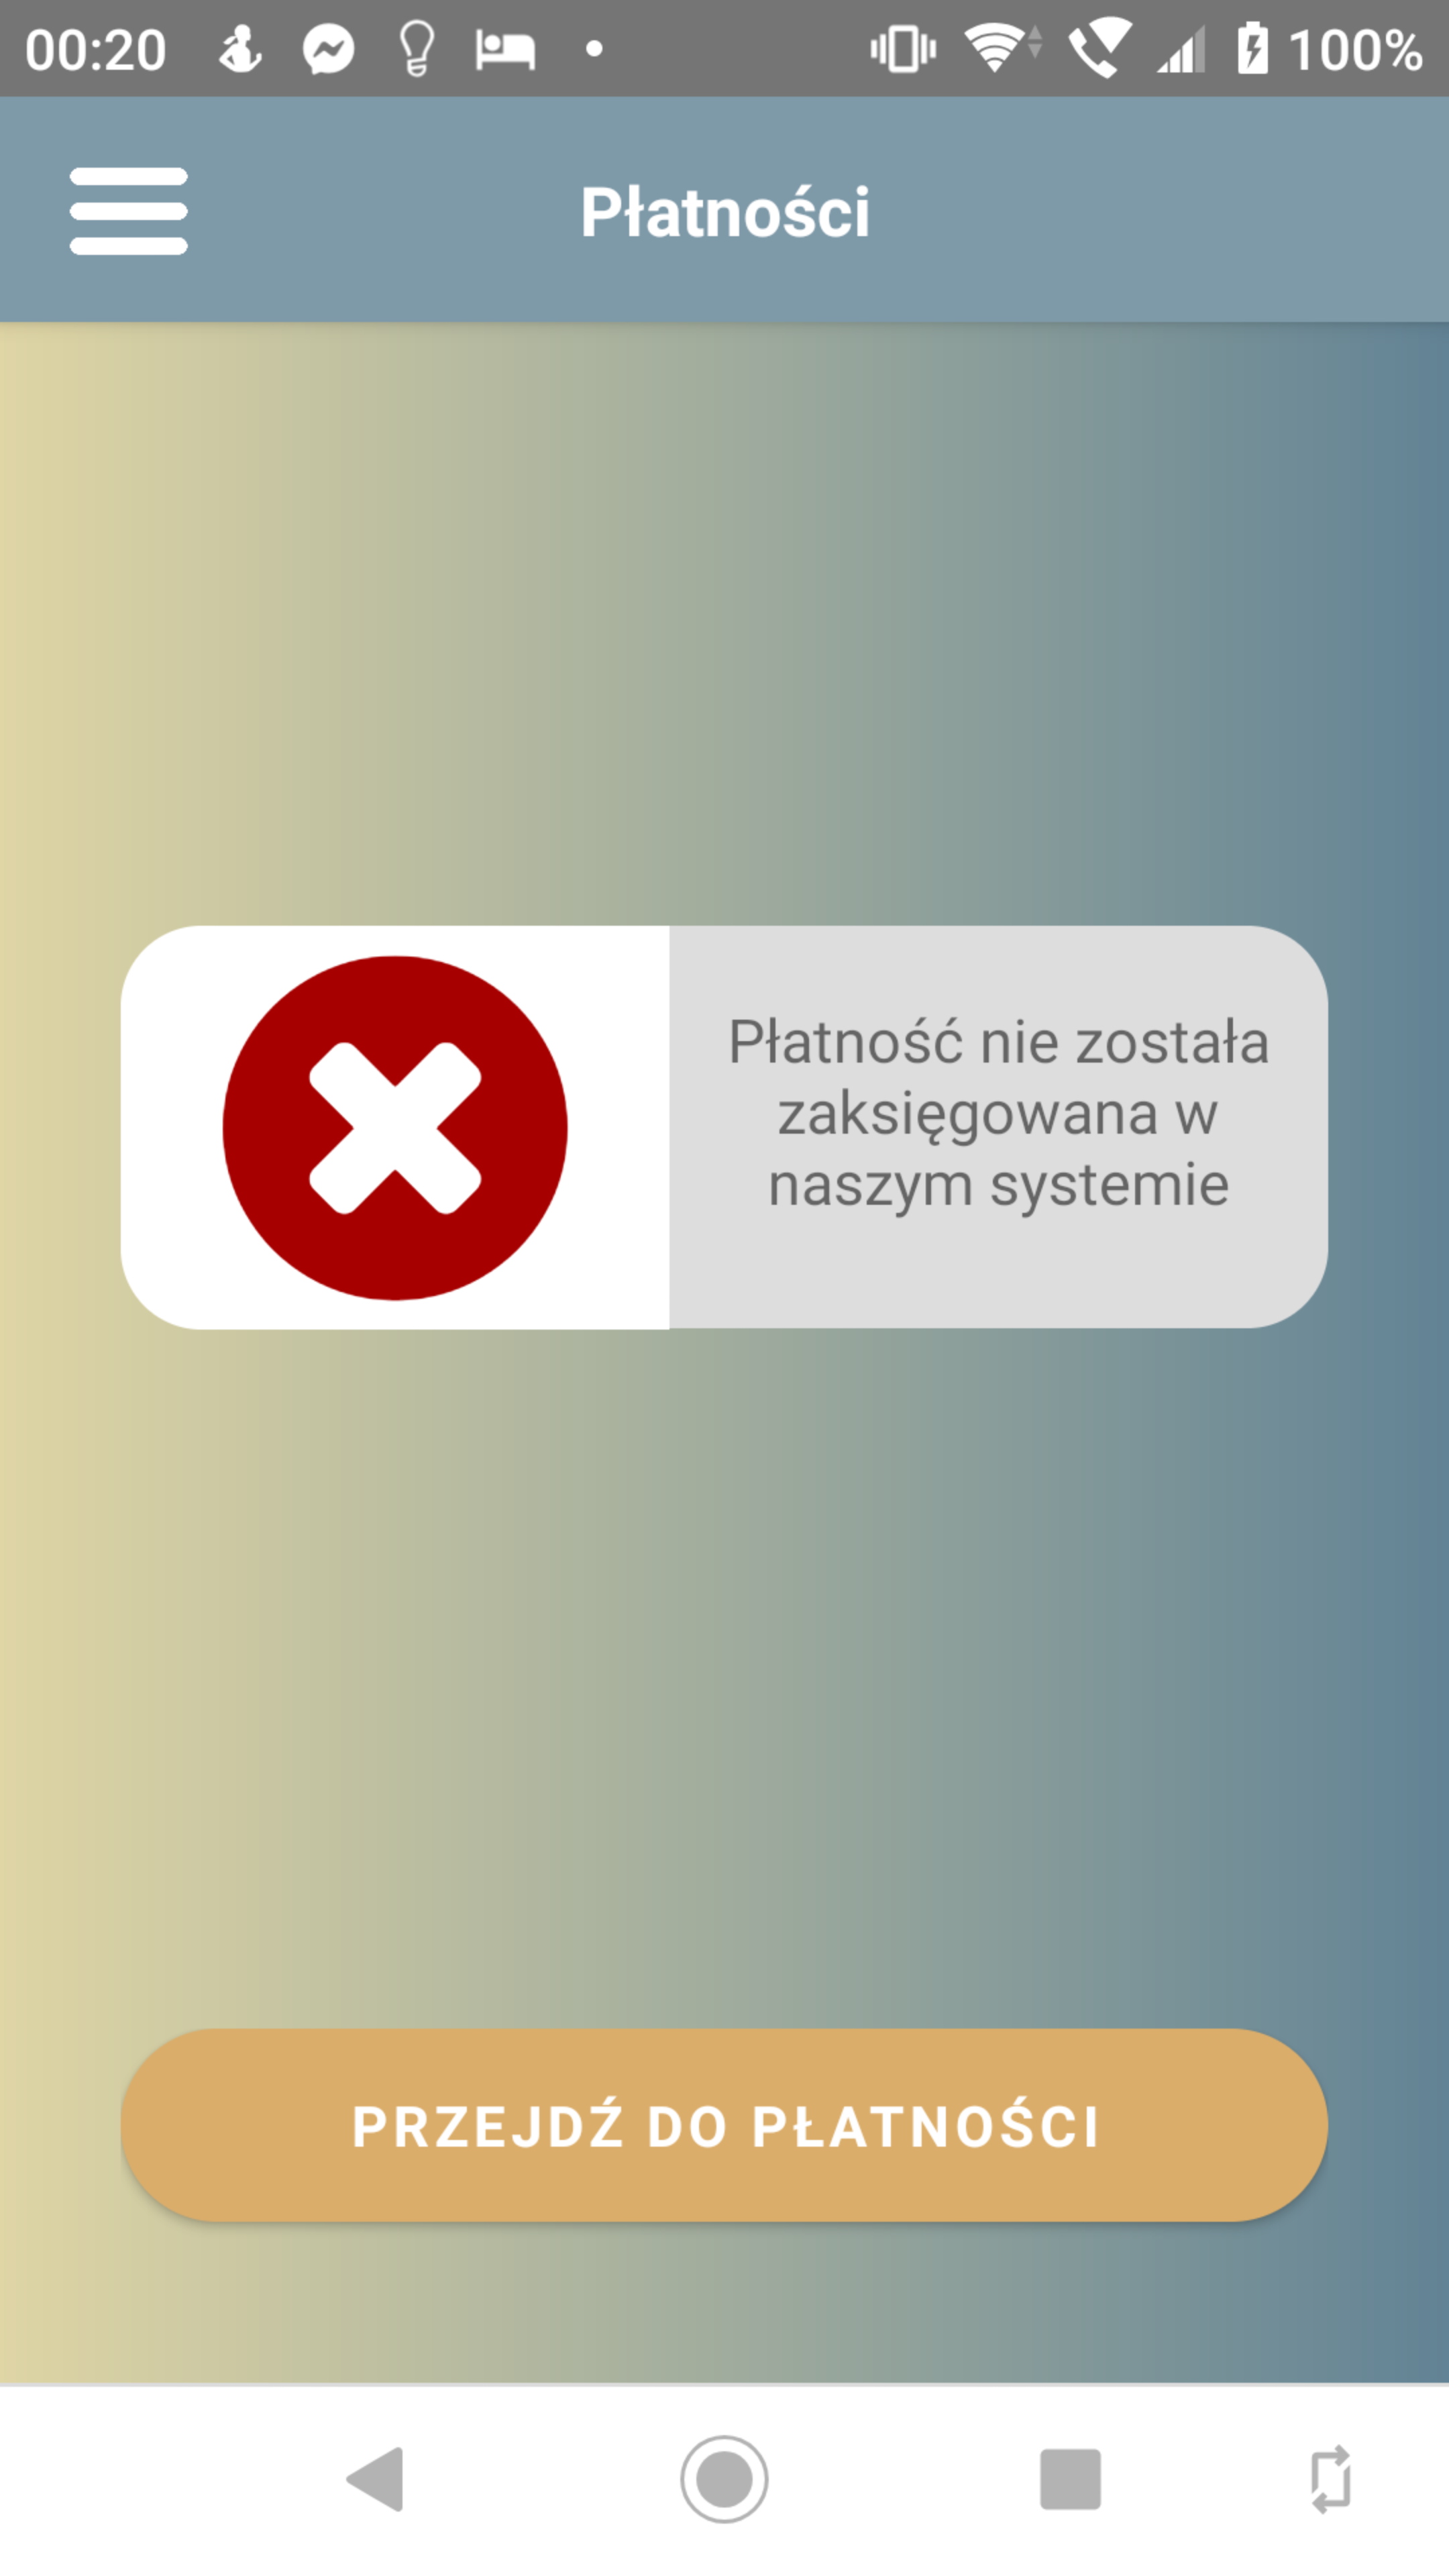
\includegraphics[width=0.45\linewidth]{images/mobile/payment.png}
    \caption{Ekran statusu płatności w aplikacji mobilnej}
    \label{fig:test3_label}
\end{figure}

\section{Panel Administratora}
Aby sprawnie zarządzać użytkownikami i egzaminami, został zbudowany panel administratora. Administrator, by skorzystać z tego panelu, musi się zalogować do systemu specjalnym loginem, otrzymanym przy wdrożeniu systemu. \\
W kolejnych podpunktach zostaną opisane operacje, jakie administrator może wykonać na kandydatach, egzaminach, kategoriach egzaminów oraz nauczycielach w systemie. Należy założyć, że jeżeli przy danej operacji nie jest napisane inaczej, to operację można wykonać dla każdej grupy wymienionej w poprzednim zdaniu.
\begin{figure}[H]
    \centering
    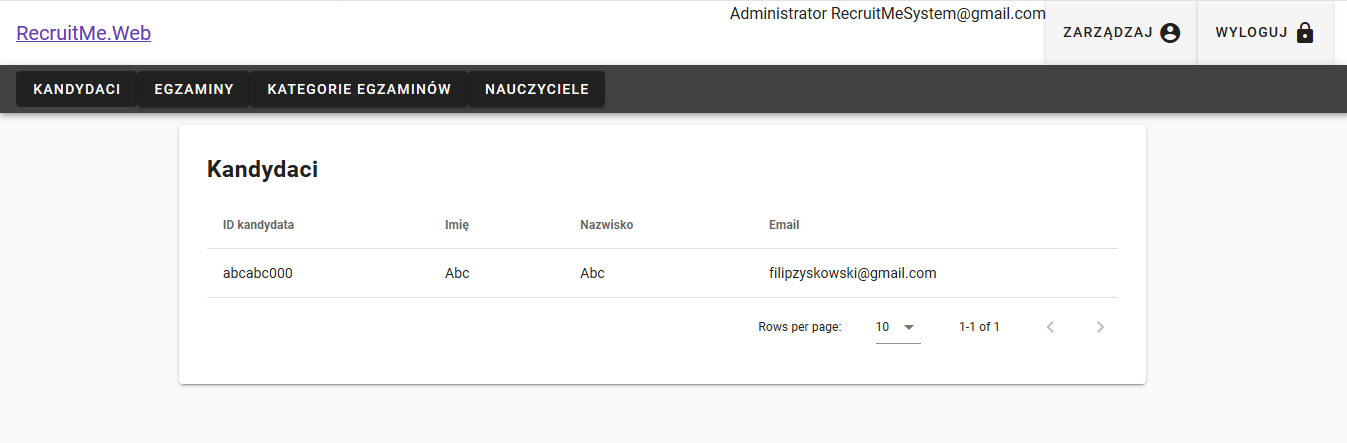
\includegraphics[width=1\linewidth]{images/web/ap_vi.png}
    \caption{Główny ekran panelu administratora}
    \label{fig:test3_label}
\end{figure}

\subsection{Dodawanie danych do systemu}
Administrator może przez panel administratora dodać nauczycieli, kategorie egzaminów i same egzaminy. Należy przejść do interesującej nas kategorii wyświetlonej na szarym pasku. Następnie należy kliknąć przycisk \emph{Dodaj} znajdujący się tuż przy nazwie danej grupy. Na koniec trzeba uzupełnić potrzebne dane i kliknąć \emph{Zapisz}.
\begin{figure}[H]
    \centering
    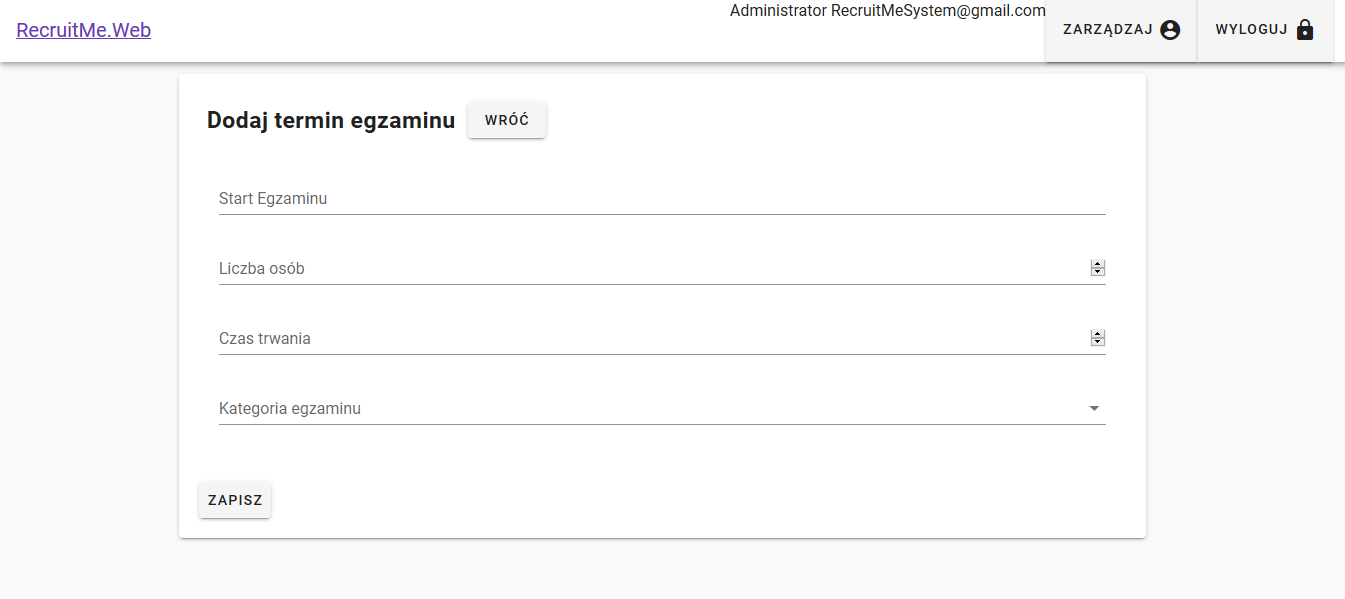
\includegraphics[width=1\linewidth]{images/web/ap_add.png}
    \caption{Przykładowe dodawanie egzaminu do systemu}
    \label{fig:test3_label}
\end{figure}

\subsection{Edycja istniejących danych}
Aby zmienić istniejące dane w systemie należy najpierw przejść do interesującej nas kategorii wyświetlonej na szarym pasku. Potem trzeba kliknąć na wybrany przez nas rekord w tabeli. Wyświetli się wtedy co najmniej jeden formularz z danymi, które możemy edytować. Na koniec edycji wystarczy kliknąć przycisk \emph{Zapisz}. \\
Trzeba uważać, by przy zmianie danych, \textbf{nie modyfikować} informacji, które uniemożliwiłyby zalogowanie się użytkownikowi.

\subsection{Usuwanie danych}
Usuwanie danych przeprowadza się w tym samym ekranie, co edycja. Gdy znajdziemy użytkownika, kategorię, egzamin lub nauczyciela, którego chcemy usunąć z systemu, wystarczy kliknąć w ekranie edycji przycisk \emph{Usuń}. Po udanym procesie, zostaniemy przekierowani na stronę danej grupy.
\begin{figure}[H]
    \centering
    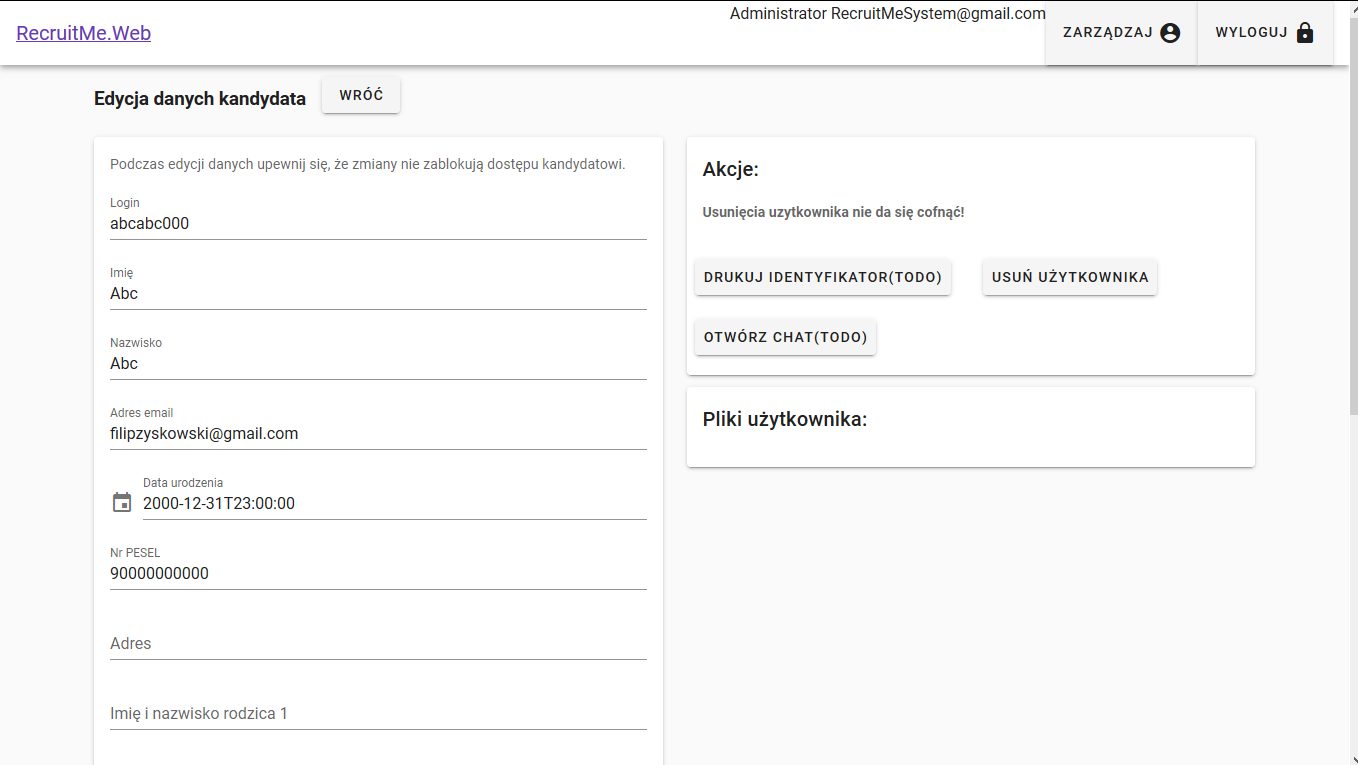
\includegraphics[width=1\linewidth]{images/web/ap_edit.png}
    \caption{Ekran edycji użytkownika}
    \label{fig:test3_label}
\end{figure}

\subsection{Drukowanie identyfikatora i chat}
Wydrukowanie identyfikatora kandydata i otworzenie okienka chatu z użytkownikiem wykonuje się w ekranie edycji użytkownika. Przechodzimy do listy użytkowników z szarego paska, klikając \emph{Kandydaci}. Wybieramy użytkownika i po prawiej stronie znajdziemy dwa przyciski: \emph{Drukuj identyfikator} oraz \emph{Otwórz chat}.

\subsection{Skanowanie ocen}
Będąc na stronie danego egzaminu możemy wydrukować kartę egzaminacyjną, za pomocą której możemy w prosty sposób wprowadzić wyniki egzaminu do systemu. Z uwagi na ograniczenie możliwości skanowania tylko jednej strony, ta funkcjonalność jest dostępna tylko dla egzaminów o co najwyżej 15 uczestnikach, co powinno wystarczyć dla egzaminów ustnych (indywidualnych), dla których ta funkcjonalność została zaprojektowana. Nauczyciel oceniający w trakcie egzaminu może zaznaczyć wynik kandydata na karcie zamalowując odpowiednie pole ciemnym kolorem (najlepiej czarnym). Zaznaczając wynik nie można wyjść poza granice pola z punktami oraz na karcie nie może być żadnych plam. Wprowadzając kartę do systemu należy zadbać aby czarna ramka była najbardziej zewnętrznym konturem na zdjęciu (lub skanie) karty. Podczas wybierania zdjęcia trzeba również podać oceniającego nauczyciela. Po czynności zaleca się sprawdzenie wprowadzonych ocen czy są zgodne z zaznaczonymi na karcie. 


\section{Historia dokumentu}

\begin{tabularx}{\linewidth}{|X|l|l|X|}
    \hline
    Autor & Data & Wersja & Wprowadzone zmiany \\
    \hline
    Filip Zyskowski & 06.01.2020 & v0.1 & Pierwsza wersja dokumentu \\
    \hline
    Andrzej Westfalewicz & 07.01.2020 & v0.2 & Dodanie opis kart egzaminacyjnych \\
    \hline
    Filip Zyskowski & 13.01.2020 & v0.3 & Uzupełnienie brakujących zdjęć i informacji z aplikacji mobilnej \\
    \hline
\end{tabularx}

\end{document}
